\documentclass[11pt,a4paper,polish,thesis]{dcsbook}

\usepackage[T1]{fontenc}
\usepackage[utf8]{inputenc}
\usepackage{babel}
\usepackage{graphicx}
\usepackage{float}

\setcounter{secnumdepth}{3}
\setcounter{tocdepth}{3}

\begin{document}

\author{Patryk Dąbrowski 100584\\ Aleksander Kędzierski 98875\\ Paweł Lampe 99277\\ Mateusz Sikora 99615}
\title{Platforma zarządzania zdarzeniami na urządzeniach mobilnych if\{y\}}
\supervisor{dr inż.~Jerzy Błaszczyński}
\date{Poznań, 2014}

\maketitle

\frontmatter

\tableofcontents{}

\mainmatter

\chapter{Wstęp}
%% Bardzo suchy wstęp zawierający to co ma być zawarte w klasycznym wstępie pracy inżynierskiej
\section{Motywacje}
Współczesne urządzenia mobilne dysponują ogromnym zbiorem modułów. Większość z nich generuje zdarzenia. Zdarzeniami mogą być przykładowo; zmiana poziomu naładowania
baterii, przychodzące połączenie czy TODO:. Niektóre zdarzenia obsługuje właściciel urządzenia, podczas gdy innymi zajmują się dedykowane aplikacje. Aby przykładowo
TODO: należy pobrać aplikację TODO:. Aplikacji podejmujących akcje w reakcji na zdarzenia jest na rynku bardzo dużo.

Wyzwanie mające na celu zbudowanie pojedynczej aplikacji do zarządzania zdarzeniami oraz akcjami zostało obecnie podjęte przez zaledwie kilka firm. Wszystkie
implementacje powstałe do tej pory są komercyjne. Hamuje to rozwój samych aplikacji jak i dziedziny. TODO: more
\section{Cele i zakres pracy}
Postawowym celem niniejszej pracy jest stworzenie otwartoźródłowej biblioteki uproszczającej dostęp do podzespołów urządzenia mobilnego. Podjeście takie ma zadanie
utworzyć warstwę abstrakcji nad systemem operacyjnym. Ma to potencjalnie zapewnić przenośność kodu pisanego przy użyciu biblioteki pomiędzy dowolnymi systemami
operacyjnymi. Niniejsza praca zakłada implementację biblioteki tylko dla systemu Android.

Pozostałe cele to stworzenie prostej aplikacji mobilnej prezentującej możliwości biblioteki oraz dwóch internetowych aplikacji pomocniczych. Fakt implementacji
biblioteki tylko dla systemu Android wymusza implementację aplikacji mobilnej również dla tego systemu operacyjnego.

Implementacja aplikacji pomocniczych jest nieunikniona ze względu na potrzebę centralizjacji niektórych danych poza obrębem pojedynczego urządzenia.

Reasumując, należy stworzyć platformę w skład której wchodzą; biblioteka dla systemu Android, aplikacja mobilna dla systemu Android oraz dwie aplikacje internetowe.
\section{Podział prac}
Podział obowiązków został dokonany na podstawie kompetencji poszczególnych osób. Częściami platformy związanymi ściśle z systemem Android zajęli się Aleksander
Kędzierski oraz Mateusz Sikora. Częściami związanymi z technologiami internetowymi zajęli się Patryk Dąbrowski i Paweł Lampe. Nad kwestiami wspólnymi dla obu części
pracował cały zespół.

Ostatecznie, poszczególne osoby dokonały:
\begin{itemize}
\item Patryk Dąbrowski
\begin{itemize}
\item text
\item text
\end{itemize}
\item Aleksander Kędzierski
\begin{itemize}
\item Zaprojektowania i implementacji części biblioteki IFY, w szczególności związanej z obsługa recept.
\item Implementacji części aplikacji appIFY.
\end{itemize}
\item Paweł Lampe
\begin{itemize}
\item Implementacji targowiska
\item Administracji serwerem z systemem Linux
\end{itemize}
\item Mateusz Sikora
\begin{itemize}
\item text
\item text
\end{itemize}
\end{itemize}
\section{Omówienie pracy}       %TODO: usunąć całą sekcję, chyba, że będzie potrzebne dodatkowe 0.5 strony A4 tekstu
%% TODO:
%% opis pracy jako dokumentu, kwestie treści etc.
%% streszczenia rozdziałów

\chapter{Wymagania}
%% wszelkie wymagania czyli:
%% wymagania funkcjonalne - to co wiemy
%% wymagania pozafuncjonalne - to czego na wstępie nie wiedzieliśmy np. 'recepty ma się łatwo pisać' - z tego w następnym rozdziale zrobi się problem który
%% został rozwiązany w postaci tych jarów
W niniejszym rozdziale zebrano wymagania funkcjonalne oraz pozafunkkcjonalne. Stanowią one opis pożądanego zachowania platformy. Wszystkie wymagania powstały
w procesie zbierania wymagań w który zaangażowany był promotor pracy oraz TODO: grupa inżynierów ze specjalizacji TWO.
\section{Wymagania funkcjonalne}
\subsection{Przypadki użycia platformy} %TODO: dodac UC dotyczace recept, usunac wszystkie UC dotyczace targowiska
\begin{description}
\item[UC1] Tworzenie Recepty
\item[1] Użytkownik wchodzi na stronę Targowiska.
\item[2]Użytkownik tworzy nową Receptę.
\item[3]Użytkownik pisze kod w edytorze online.
\item[3a]Użytkownik pisze kod lokalnie (np. w Eclipse) i przekazuje kod do Targowiska.
\item[4]Serwer kompiluje receptę.
\item[5]Użytkownik pobiera receptę na telefon.
\item[6]Recepta działa na telefonie.

\item[UC2] Ocena Recepty
\item[1] Użytkownik wchodzi na stronę Targowiska.
\item[2] Targowisko  


\end{description}
\subsection{Przypadki użycia Aplikacji - przykładowe Recepty}
\section{Wymagania pozafunkcjonalne}

\begin{tabular}{|p{2cm}|p{12cm}|}  \hline ID: &
PF01
\\ \hline Nazwa: &
System operacyjny dla aplikacji mobilnej	
\\ \hline Kategoria: &
Środowisko
\\ \hline Priorytet: &
Wysoki
\\ \hline Opis: &
Systemem operacyjnym aplikacji mobilnej jest Android w wersji minimum 2.1.

\\ \hline \end{tabular} \\\\\ \begin{tabular}{|p{2cm}|p{12cm}|}  \hline ID: &
PF02
\\ \hline Nazwa: &
Środowisko uruchomieniowe dla aplikacji serwerowej
\\ \hline Kategoria: &
Środowisko
\\ \hline Priorytet: &
Wysoki
\\ \hline Opis: &
Aplikacja serwerowa powinna działać na maszynie wirtualnej Java.

\\ \hline \end{tabular} \\\\\ \begin{tabular}{|p{2cm}|p{12cm}|}  \hline ID: &
PF03
\\ \hline Nazwa: &
Używane technologie
\\ \hline Kategoria: &
Technologie
\\ \hline Priorytet: &
Wysoki
\\ \hline Opis: &
Wykorzystane technologie nie mogą być płatne

\\ \hline \end{tabular} \\\\\ \begin{tabular}{|p{2cm}|p{12cm}|}  \hline ID: &
PF04
\\ \hline Nazwa: &
Zunifikowane środowisko programistyczne
\\ \hline Kategoria: &
Narzędzia
\\ \hline Priorytet: &
Wysoki
\\ \hline Opis: &
Programiści muszą zdecydować się na wspólne narzędzie do redagowania kodu (np. Eclipse)

\\ \hline \end{tabular} \\\\\ \begin{tabular}{|p{2cm}|p{12cm}|}  \hline ID: &
PF05
\\ \hline Nazwa: &
Ograniczone zużycie energii urządzenia mobilnego
\\ \hline Kategoria: &
Wydajność i niezawodność
\\ \hline Priorytet: &
Średni
\\ \hline Opis: &
Działanie aplikacji nie powinno w znaczącym stopniu skracać czasu pracy urządzenia na baterii

\\ \hline \end{tabular} \\\\\ \begin{tabular}{|p{2cm}|p{12cm}|}  \hline ID: &
PF06
\\ \hline Nazwa: &
Ograniczone zużycie zasobów urządzenia mobilnego.
\\ \hline Kategoria: &
Wydajność i niezawodność
\\ \hline Priorytet: &
Średni
\\ \hline Opis: &
Aplikacja nie powinna spowalniać działania innych aplikacji.

\\ \hline \end{tabular} \\\\\ \begin{tabular}{|p{2cm}|p{12cm}|}  \hline ID: &
PF07
\\ \hline Nazwa: &
Czas reakcji aplikacji na zdarzenie
\\ \hline Kategoria: &
Wydajność i niezawodność
\\ \hline Priorytet: &
Wysoki
\\ \hline Opis: &
Aplikacja powinna reagować na zdarzenia lokalne w mniej niż 2 sekundy

\\ \hline \end{tabular} \\\\\ \begin{tabular}{|p{2cm}|p{12cm}|}  \hline ID: &
PF08
\\ \hline Nazwa: &
Zgodność ze standardami kodowania dla języka Java
\\ \hline Kategoria: &
Zgodność ze standardami
\\ \hline Priorytet: &
Wysoki
\\ \hline Opis: &
Zarówno kod aplikacji mobilnej, jak i serwerowej powinien być redagowany zgodnie ze standardami dla języka Java

\\ \hline \end{tabular} \\\\\ \begin{tabular}{|p{2cm}|p{12cm}|}  \hline ID: &
PF09
\\ \hline Nazwa: &
Przechowywanie haseł
\\ \hline Kategoria: &
Bezpieczeństwo
\\ \hline Priorytet: &
Wysoki
\\ \hline Opis: &
Szyfrowane zapamiętywanie hasła użytkownika.

\\ \hline \end{tabular} \\\\\ \begin{tabular}{|p{2cm}|p{12cm}|}  \hline ID: &
PF10
\\ \hline Nazwa: &
Przechowywanie haseł
\\ \hline Kategoria: &
Bezpieczeństwo
\\ \hline Priorytet: &
Wysoki
\\ \hline Opis: &
Przechowywanie skrótu hasła na serwerze.
\\ \hline \end{tabular} \\\\\ \begin{tabular}{|p{2cm}|p{12cm}|}  \hline ID: &
PF11
\\ \hline Nazwa: &
Długość recepty
\\ \hline Kategoria: &
Użyteczność
\\ \hline Priorytet: &
Wysoki
\\ \hline Opis: &
Długość kodu recepty nie powinna w średnim przypadku przekraczać 100 linii
\\ \hline \end{tabular} \\\\\ \begin{tabular}{|p{2cm}|p{12cm}|}  \hline ID: &
PF12
\\ \hline Nazwa: &
Tworzenie recept
\\ \hline Kategoria: &
Użyteczność
\\ \hline Priorytet: &
Wysoki
\\ \hline Opis: &
Proces tworzenia recepty nie powinien zajmować więcej niż 15 minut
\\ \hline \end{tabular} \\\\\ \begin{tabular}{|p{2cm}|p{12cm}|}  \hline ID: &
PF13
\\ \hline Nazwa: &
Dystrybucja recept
\\ \hline Kategoria: &
Użyteczność
\\ \hline Priorytet: &
Średni
\\ \hline Opis: &
Proces dystrybucji recepty nie powinien zajmować więcej niż 5 minut
\\ \hline \end{tabular} \\\\\ \begin{tabular}{|p{2cm}|p{12cm}|}  \hline ID: &
PF14
\\ \hline Nazwa: &
Bezpieczeństwo recept
\\ \hline Kategoria: &
Bezpieczeństwo
\\ \hline Priorytet: &
Wysoki
\\ \hline Opis: &
Recepta powinna korzystać tylko z biblioteki if\{y\} oraz pakietów narzędziowych Java
\\ \hline \end{tabular}

\chapter{Zarządzanie zdarzeniami na urządzeniach mobilnych}
%% wstęp vol. 2 - naświetlanie aktualnej wiedzy na temat tego co robimy, tutaj definiujemy pojęcia pokazujemy inne rozwiązania, ciśniemy po nich etc.
Jak wspomniano w rozdziale 1, zarządzanie zdarzeniami na urządzeniach mobilnych doczekało się zaledwie kilku implementacji ze strony zainteresowanych firm.
Tematyka jest więc otwarta zarówno na pomysły jak i terminologię.

W niniejszym rozdziale wprowadzono przede wszystkim pojęcia które pojawiają się w dalszych częściach pracy. Dokonano również przeglądu istniejących rozwiązań
pod kątem mocnych oraz słabych stron.

\section{Definicja pojęć}
\begin{itemize}
\item Podfunkcjonalność (ang. Feature) -- Część biblioteki zapewniająca Receptom dostęp do pozdbioru funkcjonalności Androida.
\item Zdarzenie (ang. Event) -- Zmiana stanu systemu, która powoduje uruchomienie kodu Recepty.
\item Recepta (ang. Recipe) -- Napisany przez użytkownika fragment kodu opisujący, co ma się zdarzyć po spełnieniu pewnych warunków.
\item Targowisko (ang. Market) -- Aplikacja internetowa pozwalająca tworzyć i pobierać Recepty.
\item Aplikacja Kliencka -- Aplikacja androidowa wykorzystująca bibliotekę if\{Y\}. 
\item Serwer Grup -- Komputer z działającą aplikacją, która zarządza grupami użytkowników i Zdarzeniami Grupowymi.
\item Zdarzenie Grupowe -- Zdarzenie związane z Grupą, wysyłane lub odbierane przez Aplikację z Serwera Grup.
\item Grupa -- Zbiór użytkowników identyfikowalny przez nazwę zdefiniowany na Serwerze Grup.
\item Dziennik (ang. Log) -- Moduł systemu odpowiedzialny za zapis zdarzeń.
\end{itemize}
\section{Istniejące rozwiązania} %TDOO mocne strony / słabe strony !
\subsection{On X}
Aplikacja firmy Microsoft umożliwiającą kontrolowanie telefonu z systemem Android używając kodu napisanego w JavaScript. Umożliwia wysyłanie Zasad (and. Rules) na
telefon poprzez stronę internetową. Dostęp do funckcjonalości systemu Android jest zapewniony przez API w postaci Wyzwalaczy (ang. Triggers) i Akcji (ang. Actions).
Cały system jest [niestety] połączony z Facebookiem i wymaga posiadania tam konta. Na podstawie \cite{onx}.
\subsection{Tasker}
TODO:

\chapter{Architektura platformy}
%% WYSOKI POZIOM ABSTRAKCJI ! Opis problemów, koncepcje rozwiązań, UMLe Diagramy Encji etc.
System składa się z biblioteki IFY, przykładowej aplikacji appIFY oraz aplikacji działających na serwerze - Serwera Grup oraz Targowiska.
Biblioteka zawiera moduł zarządzania receptami i zbiór Podfunkcjonalności.
Aplikacja korzysta z biblioteki, umożliwia przeglądanie zasobów Targowiska i zarządzanie grupami. 
Targowisko umożliwia przechowywanie Recept i tworzenie ich z poziomu przeglądarki.
Serwer grup zapewnia komunikację między Receptami na różnych urządzeniach w ramach grupy oraz zarządzanie grupami.

\section{Recepty}
Miejscem, gdzie zdefiniowana jest właściwe działanie Aplikacji są Recepty -- są w nich opisane wszystkie zdarzenia, które mają nastąpić po spełnieniu pewnych warunków. Docelowo będą one tworzone przez użytkowników i pobierane z Targowiska, jednak istnieją także przykładowe Recepty wbudowane w Aplikację, mające na celu ułatwienie użytkownikom tworzenia nowych na ich podstawie oraz rozszerzenie początkowej funkcjonalności aplikacji. 
Na receptę składają się:
\begin{itemize}
\item  opis używanych podfunkjonalności
\item  opis wymaganych parametrów
\item  opis jej właściwego działania
\end{itemize}
Deklarowanie używanych podfunkcjonalności ma dwa główne cele - po pierwsze, użytkownik widzi, czego używa recepta, co nieco poprawia jego bezpieczeństwo przy używaniu recept innych użytkowników, po drugie pozwala to inicjalizować nasłuchiwanie zdarzeń systemowych tylko wtedy, gdy istnieje aktywna recepta, która na nie reaguje - kod recepty nie musi inicjalizować większości podfunkcjonalności, wystarczy deklaracja ich używania. Wyjątkiem jest podfunkcjonalność grup, gdzie komunikację należy zainicjalizować.

Parametry pozwalają użytkownikowi na dostosowanie recepty do swoich wymagań, bez potrzeby pisania nowej. W naszych przykładowych receptach były to np. numer telefonu do wysłania SMS lub jego tekst czy też zasięg znajdowania znajomych na podstawie GPS.
Właściwa logika recepty jest zawarta w funkcji reakcji na zdarzenie. Jest to rozwiązanie podobne do wzorca obserwatora, Recepta staje się jednak obserwatorem automatycznie na podstawie zadeklarowanych podfunkcjonalności, co pozwala zmniejszyć ilość kodu w receptach.

\subsection{Cykl życia}
W konstekście platformy if\{y\} zdefiniować można następujący cykl życia recepty:
\begin{enumerate}
\item Pisanie kodu
\item Kompilacja i budowa
\item Dystrybucja
\item Pobranie na urządzenie mobilne
\item Uruchomienie
\item Działanie
\end{enumerate}

\subsection{Recepty Grupowe}
Główną ideą recept grupowych jest działanie jednocześnie na wielu urządzeniach, tak, aby zdarzenia na jednym urządzeniu mogły wpływać na drugie. Zatem komunikacja jest możliwa między instancjami  tej samej recepty na różnych urządzeniach. Jest ona możliwa na dwa sposoby:
\begin{itemize}
\item{Wysyłanie zdarzeń}\\
Polega na utworzeniu zdarzenia, które jest obsługiwane na innym urządzeniu, które nasłuchuje go automatycznie.
\item{Wysyłanie danych}\\
Polega na wysyłaniu na serwer danych, które potem mogą być odczytane na innym urządzeniu.
\end{itemize}
Nie da się natomiast napisać w Recepcie kodu, który byłby wywoływany na serwerze. Kłóciłoby się to z prostotą mechanizmu recepty - musiałaby się ona składać zarówno z kodu dla aplikacji, jak i dla serwera, a programista musiałby zadbać o ich współpracę. Mogłoby to też stanowić zagrożenie dla stabilności serwera w wypadku złośliwego kodu.
Nie udało się też znaleźć scenariuszy użycia, w których taka funkcja byłaby konieczna. Dodatkowo przyjęta architektura pozwala na odseparowanie Serwera Grup od Targowiska. 

\section{Biblioteka}
Biblioteka zawiera API dostępne z poziomu recept, czyli między innymi Podfunkcjonalności, które agregują i upraszaczają dostęp do metod z API systemu Android oraz umożliwiają reagowanie na zdarzenia zachodzące na urządzeniu mobilym.
Istotnym elementem Biblioteki jest moduł zarządzający cyklem życia Recept i Podfunkcjonalności. W kontekście Biblioteki, cykl życia Recepty wygląda tak jak na rysunku
\ref{fig:cykl-zycia-recepty}.
\begin{figure}[H]
  \centering
  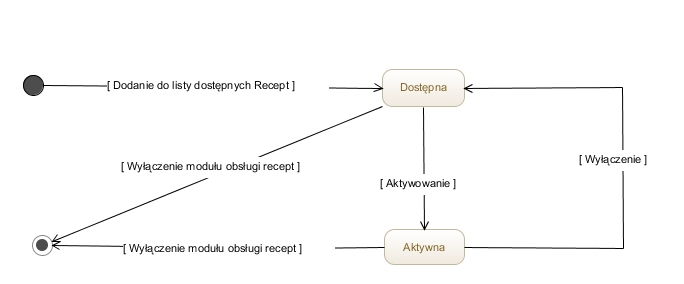
\includegraphics[scale=0.6]{./resources/cykl-zycia-recepty.jpg}
  \caption{Cykl życia recepty z punktu widzenia biblioteki}
  \label{fig:cykl-zycia-recepty}
\end{figure}
Wyróżniamy dwa stany w których znajdują się Recepty:
\begin{itemize}
\item Dostępna - udostępnia podstawowe informacje - nazwę, zbiór parametrów potrzebnych do uruchomienia i deklaracje Podfunkcjonalności, z którch będzie korzystać.
\item Aktywna - została uruchomiona na urządzeniu mobilnym, działa cały czas w tle nasłuchując na Zdarzenia, podczas jej uruchamiania zostały podane parametry i przydzielone Podfuncjonalności.
\end{itemize}
Warto zauważyć, że możliwe jest uruchomienie wielu instancji tej samej Recepty - mogą się różnić nadanymi parametrami.
Cykl życia Podfunkcjonalności jest ściśle związany z Receptami - dana Podfunkcjonalność jest aktywna w systemie tylko jeżeli istnieją aktywne Recepty, które z niej korzystają. 
Moduł zarządzania Receptami aktywuje Podfunkcjonalność podczas uruchamiania pierwszej Recepty która zadeklarowała jej użycie i wyłącza ją kiedy nie pozostaną w systemie żadne aktywne Recepty które mogłby z niej korzystać.
Podczas wyłączania zwalniane są wykorzystywane zasoby. Biblioteka zawiera również mechanizm komunikacji z Aplikacjami Klienckimi. Podczas projektowania wzięto pod uwagę zapewnienie rozszerzenia istniejącego zbioru Podfunkcjonalności.
Moduł zarządzania Receptami składa się z listy aktywnych i dostępnych Recept oraz wykorzystywanych Podfunkcjonalności.
\begin{figure}[H]
  \centering
  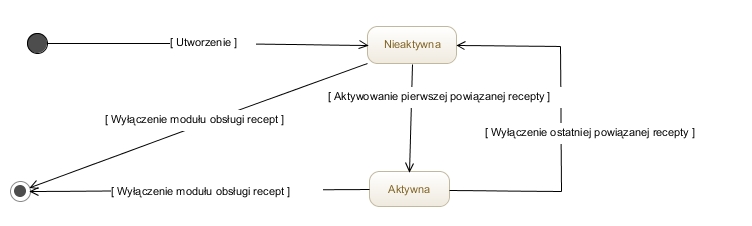
\includegraphics[scale=0.6]{./resources/cykl-zycia-featurea.jpg}
  \caption{Cykl życia podfunkcjonalności}
  \label{fig:cykl-zycia-featurea}
\end{figure}

\section{Aplikacja appIFY}
Aplikacja appIFY stanowi interfejs graficzny biblioteki - umożliwia dostęp do listy dostępnych i aktywnych Recept, ustalanie ich parametrów przy włączaniu i wyłączanie. Umożliwia korzystanie z zasobów Targowiska. Zapewnia możliwość zarządzania grupami użytkowników korzystająć z API wystawionego przez Serwer Grup.
W Aplikacji rozszerzono funkcje modułu obsługi Recept - możliwe jest wykorzystywanie tych pobranych z Targowiska i zapisywanie stanu aktywnych recept w bazie danych, co było potrzebne ze wzlędu na mechanizm zarządzania zasobami w systemie Android - każdy proces może zostać zatrzymany w dowolnej chwili, dlatego potrzebny był sposób na odtworzenie stanu Aplikacji sprzed zamknięcia. Zmodyfikowany cykl życia Recepty przedstawia rysunek \ref{fig:cykl-zycia-recepty-appify}.
\begin{figure}[H]
  \centering
  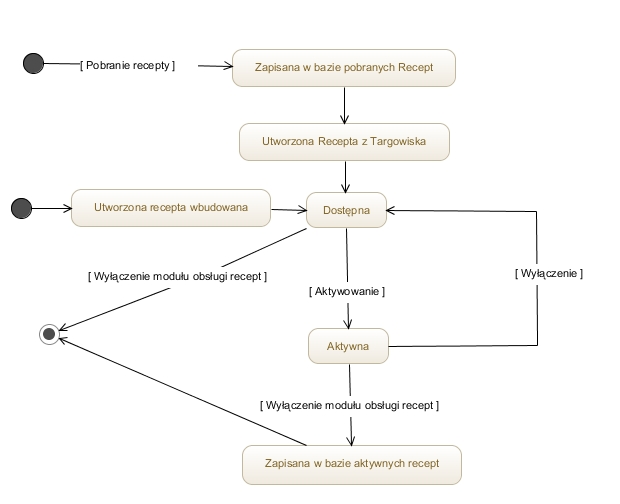
\includegraphics[scale=0.7]{./resources/cykl-zycia-recepty-appify.jpg}
  \caption{Cykl życia recepty w appIFY}
  \label{fig:cykl-zycia-recepty-appify}
\end{figure}

\section{Targowisko}
Podrozdział 2.2 definiuje zbiór wymagań pozafunkcjonalnych. Wymagania bezpośrednio dotyczące recept takie jak PF12 czy PF13 są w praktyce niemożliwe do zrealizowania
na aplikacji mobilnej. W związku z powyższym postanowiono stworzyć aplikację pomocniczą realizującą w praktyce pierwsze trzy fazy cyklu życia recepty w
ramach określonych przez wymagania pozafunkcjonalne.

Pierwsze trzy fazy cyklu życia recepty to kolejno:
\begin{enumerate}
\item Pisanie kodu
\item Kompilacja i budowa
\item Dystrybucja
\end{enumerate}

Pierwsze dwa punkty powyższej listy można zrealizować poprzez dostarczenie zintergrowanego środowiska programistycznego. Trzeci, poprzez stworzenie aplikacji
internenetowej korzystającej z bazy danych. Powstało więc Targowisko -- aplikacja internetowa przypominająca nieco Google Play, z dodatkowymi funkcjami.
Pierwszą z nich jest stworzenie zintegrowanego środowiska programistycznego wbudowanego bezpośrednio w Targowisko. Drugą, zastosowanie idei rozwidlania Recept.

\subsection{Zintegrowane środowisko programistyczne}
%% TODO: 0 informacji IMO
%% Współcześnie, wiele złożonych usług dostępnych jest z poziomu przeglądarki internetowej. Podejście takie wiąże się z pojęciem chmury -- modelu przetwarzania danych, gdzie ciężar przetwarzania przenoszony jest na serwer. O chmurze jako bazie dla Google Play, Jamie Rosenberg napisał w \cite{googleplay}. W targowisku postanowiono wykorzystać ten model. Właśnie dlatego, zintegrowane środowisko programistyczne postanowiono wbudować w aplikację internetową.

Pomysł zakładał osadzenie edytora na stronie internetowej. Strona ta posiadałaby jednocześnie mechanizmy umożliwiające kompilację i budowę kodu recepty. Oczekiwanym
plikiem powstawałym na wyjściu tego procesu byłoby archiwum Java (\emph{jar}) gotowe do wgrania na aplikację kliencką if\{y\}.

Okazuje się, że istnieją darmowe edytory kodu nadające się do umieszczenia na stronie. Co więcej, wywoływanie komend systemu operacyjnego z poziomu aplikacji
internetowej również okazało się w pełni możliwe. Wybrano więc napisany w JavaScript edytor Ace -- z racji na najlepszą dokumnetację oraz język PHP który
świetnie radzi sobie również z zadaniami niskiego poziomu.
\subsection{Rozwidlanie}
Pierwotne założenie dotyczące budowania nowych recept zakładało istnienie generatora kodu. Miał on na celu umożliwienie wygenerowania części kodu w zależności od
wybranych przez użytkownika, podfunkcjonalności z biblioteki if\{y\}. Generator taki był dyskusyjny z powodu pracochłonnej implementacji oraz specyfiki biblioteki.
Generator powinno implementować się po ostatecznej implementacji biblioteki. Biblioteka jednak z założenia jest kodem który dynamicznie rozwija się w czasie.

Ostatecznie, zamiast generatora, postanowiono wykorzystać ideę rozwidlania (ang. fork). Idea ta w praktyce oferuje prawie to samo co generator kodu. Istnieje jednak
jedna spora różnica. Rozwidlanie pielęngnuje się samo w sobie. Wystarczy stworzyć jeden działający kawałek kodu i opublikować go. Od tego momentu, każdy może zacząć pisanie swojego kodu przyjmując jako punkt wyjścia kod opublikowany wcześniej. Proces ten może powtarzać się rekursywnie w nieskończoność.

Stosowane podeście nie jest wolne od wad. Kluczową może być fakt, iż działający kod niskiej jakości może być niepotrzebnie propagowany. Propagacja może się też tyczyć
wysokiej jakości kodu, przez co problem propagacji w ogólności można uznać za mało szkodliwy.
\subsection{Repozytorium recept}
Zarządzanie receptami postanowiono zrealizować angażując strukturę katalogową targowiska oraz bazę danych. Pliki ze zbudowanym kodem zgromadzono w katalogu \emph{jar}.
Wszelkie informacje pomocnicze umieszczono w bazie danych o schemacie widocznym na rysunku \ref{fig:market_db}, gdzie:
\begin{figure}[p]
  \centering
  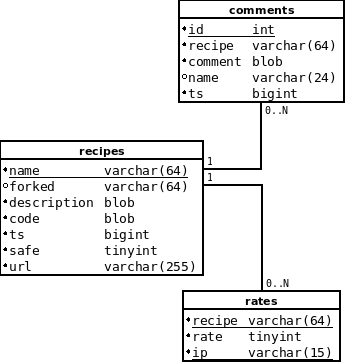
\includegraphics[scale=0.7]{./resources/market_db.png}
  \caption{Schemat bazy danych targowiska}
  \label{fig:market_db}
\end{figure}
\begin{itemize}
\item recipes -- jest to relacja której każda krotka utożsamiana jest z pojedyńczą receptą. Każda recepta posiada własną, unikalną nazwę, opcjonalnie nazwę recepty
z której dana została wywiedziona, opis, kod źródłowy, znacznik czasu dodania, flagę informującą o niebezpiecznych konstrukcjach w kodzie oraz łącze do pliku
\emph{jar}.
\item comments -- jest to relacja której krotki reprezentują komentarze użytkowników na temat recept. Każdy komentarz posiada unikalny identyfikator liczbowy, nazwę
recepty której się tyczy, treść komentarza, opcjonalnie nazwę autora oraz znacznik czasu dodania.
\item rates -- jest to relacja której krotki reprezentują oceny w całkowitej skali od 1 do 5 przyznawane receptom. Na każdą ocenę składa się nazwa recepty ocenianej,
wartość całkowitoliczbowa oceny oraz adres IP oceniającego.
\end{itemize}
Stworzono także interfejs programowania aplikacji (API). Ma on na celu umożliwienie dostępu do targowiska z poziomu aplikacji klienckiej if\{y\}. Interfejs ten
pozwala na uzyskanie całej zawartości bazy danych w formacie JSON.
\section{Serwer Grup}
Głównym zadaniem Serwera Grup jest przekazywanie wiadomości umożliwiajęcych komunikację miedzy klientami i wymianę danych. 
Informacje te powinny być jednocześnie rozsyłane w prosty i łatwy do odczytania sposób przez każdą ze stron.
Bezpośrednia komunikacja z użyciem połączenia internetowego między urządzeniami mobilnymi nie jest możliwa, dlatego niezbędnym było wprowadzenie urządzenia pośredniczącego w przesyłaniu danych. 
Rozwiązaniem tego problemu mogła być usługa Google Cloud Messaging(GCM), lecz nie spełniała jednych z założeń projektu o odseparowaniu aplikacji od sieci społecznościowych i isniejących serwisów.
Kolejna koncepcja opiera się o tak zwany mechanizm odpytywania (ang. polling), który jest prosty do zaimplementowania, a jednocześnie spełnia wszytskie wymagania stawiane w projekcie - odbieranie danych z serwera wykonywane poprzez cykliczne zapytania eliminuje problem łączności między aplikacja a pośredniczącym serwerem.
Innym z pomysłów było wykorzystanie protokołu MQTT (MQ Telemetry Transport), który jest jednak trudny w implementacji i prawdopodobnie zwiększyłby liczbę używanych bibliotek, nie przynosząc większych korzyści w porównaniu z odpytywaniem.
Istotnym aspektem w wymianie danych między użytkownikami są ograniczenia do komunikacji aby niemożliwe było otrzymanie wiadomości od niezidentyfikowanego użytkownika.
Rozwiązanie jest połaczenie użytwkoników w grupy, w obrębie których będa mogli rozsyłać wiadomości. W zwiazku z tym serwer musi także umożliwiać zarządzanie grupami.

\chapter{Opis implementacji}
%% NISKI POZIOM ABSTRAKCJI - detale techniczne - technologie, dokumnetacje, narzędzia, KOD, KOD, jeszcze trochę KODU, jakieś tricki w KODZIE etc.

\section{Recepty}
%% TODO: ref PF11 (jar)
Recepty dziedziczą po klasie abstrakcyjnej YRecipe i implementują jej abstrakcyjne metody. Obrazuje to poniższy przykład recepty, która odrzuca wszystkie nadchodzące połączenia i wysyła SMS o zdefiniowanej przez użytkownika treści do dzwoniącej osoby.

\begin{verbatim}
public class YSampleCallsSMS extends YRecipe {
   @Override
   public void requestParams(YParamList params) {
      //Message to send in SMS
      params.add("MSG",YParamType.String, "Sorry, I'm busy.");
   }

   @Override
   public long requestFeatures() {
      return Y.Calls | Y.SMS;
   }

   @Override
   public void handleEvent(YEvent event) {
      //event is incoming call
      if(event.getId() == Y.Calls){
         YCallsEvent e = (YCallsEvent) event;
         //extract phone number
         String phone = e.getIncomingNumber();
         //discard call
         mFeatures.getCalls().discardCurrentCall();
         //send sms
         mFeatures.getSMS().sendSMS(phone, mParams.getString("MSG"));
      }
   }
   @Override
   public String getName() {
      return "YSampleCallsSMS";
   }
   @Override
   public YRecipe newInstance() {
      return new YSampleCallsSMS();
   }
}
\end{verbatim}
\subsection{Parametry -- requestParams}
Metoda requestParams ma za zadanie poinformować, jakich parametrów recepta wymaga do działania. Początkowo miała ona po prostu zwrócić listę i wyglądałaby tak:
\begin{verbatim}
public void requestParams() {
   YParamList params = new YParamList();
   params.add("MSG",YParamType.String, "Sorry, I'm busy.");
   return params;
}
\end{verbatim}
jednak tworzenie listy i zwracanie jej to dwie linie, które byłyby identyczne w każdej recepcie - ich wpisywanie może nieco irytować. Wobec tego obecnie metoda ta przyjmuje jako argument pustą listę parametrów, którą ma za zadanie wypełnić, zgodnie z założeniem maksymalnego uproszczenia kodu recepty.

\subsection{Używane Podfunkcjonalności -- requestFeatures}
Metoda requestFeatures ma za zadanie poinformować system, jakich Podfunkcjonalności używa Recepta. Początkowo była ona podobna do requestParams i wypełniała listę nowymi obiektami odpowiedniej klasy, co wyglądałoby tak:
\begin{verbatim}
public void requestFeatures(YFeatureList features) {
   features.add(new YCallsFeature());
   features.add(new YSMSFeature());
   return params;
}
\end{verbatim}
Przy takim rozwiązaniu jednak tworzyło się wiele niepotrzebnych obiektów - poprawnie zainicjalizowane Podfunkcjonalności powinny być tworzone w systemie tylko raz. Wystarczyłaby zatem lista identyfikatorów, pozwalająca zainicjalizować odpowiednie Podfunkcjonalności. Identyfikatorów jest jednak na tyle mało, że tak naprawdę nie potrzeba prawdziwej listy, wystarczy maska bitowa. Ułatwia to przesyłanie takiej listy między modułami systemu, działającymi w różnych procesach - nie trzeba się martwić o implementację w liście interfejsu Parcelable, potrzebnego do przesyłania obiektów między procesami w Androidzie.

Ostatecznie zatem metoda ta zwraca liczbę typu long, będącą sumą bitów reprezentujących poszczególne Podfunkcjonalności. Mapowanie tych bitów jest zawarte w klasie Y.
\begin{verbatim}
[...]
public static final long Wifi = 0x0008;
public static final long GPS = 0x00010;
[...]
\end{verbatim}
Dodatkowo warto zauważyć, że nazwy stałych w tej klasie odpowiadają nazwom Podfunkcjonalności oraz Zdarzeń - dla stałej {\bf ABC} klasa z Podfunkcjonalnością nazywa się Y{\bf ABC}Feature, a zdarzenie - Y{\bf ABC}Event. Powinno to ułatwić automatyczne generowanie kodu recept. 

\subsection{Logika recept -- handleEvent}
Metoda jest wywoływana, gdy w systemie nastąpi zdarzenie związane z Podfunkcjonalnością używaną przez receptę. W argumencie podawane jest zdarzenie -- obiekt typu YEvent. 
Aby poznać szczegóły zdarzenia recepta musi sprawdzić jego typ porównując wartość zwracaną przez getId() ze stałymi z klasy Y. Następnie można zrzutować zdarzenie na odpowiedni typ i poznać jego szczegóły. 

%Niestety nie udało się tutaj znaleźć bardziej eleganckiego rozwiązania. 
Recepty mogą też zażądać pewnych danych od systemu, które są dostarczane asynchronicznie - na przykład przetłumaczenie danych z GPS na adres (Geocoder). Wyniki tego typu operacji również są przekazywane do recepty jako typ YEvent.

Z poziomu obsługi zdarzenia można także dostać się do listy Podfunkcjonalności oraz listy Parametrów poprzez metody getFeatures() i getParams(). Początkowo dostęp do Podfunkcjonalności odbywał się następująco:
\begin{verbatim}
YCallsFeature cf = (YCallsFeature) mFeatures.get(Y.Calls);
\end{verbatim}
Jednak wymuszało to rzutowanie i niepotrzebnie wydłużało kod, zatem obecnie klasa YFeatureList zawiara metody pobierające konkretne podfuncjonalności.
\begin{verbatim}
public YCallsFeature getCalls() {
    return (YCallsFeature) get(Y.Calls);
}
\end{verbatim}
Ich utrzymanie może być później nieco kłopotliwe - każde dodanie Podfunkcjonalności będzie wymagało dodania odpowiedniej metody, jednak uproszczenie kodu recepty jest tego warte.

Warto również wspomnieć, że metoda handleEvent może rzucić dowolny wyjątek - recepta zostanie wówczas wyłączona. Ułatwia to pisanie recept zapewniając jednocześnie stabilność aplikacji.

\subsection{Aktywacja}
Fragmenty kodu przedstawione poniżej różnią się od oryginalnych -- dla poprawy czytelności nie ma w nich tworzenia logów.
Recepta jest aktywowana przez serwis, na podstawie nazwy i listy parametrów.
\begin{verbatim}
   public int enableRecipe(String name, YParamList params) {
      int id = ++mRecipeID;
      int timestamp = (int) (System.currentTimeMillis() / 1000);
      YRecipe recipe = mAvailableRecipesManager.getRecipe(name).newInstance();
      long feats = recipe.requestFeatures();
      YFeatureList features = new YFeatureList(feats);
      initFeatures(features);
      params.setFeatures(feats);
      if(!recipe.initialize(this, params, features, id, timestamp)){
         return 0;
      }
      for (Entry<Long, YFeature> entry : features) {
         entry.getValue().registerRecipe(recipe);
      }
      mActiveRecipesManager.put(id, recipe);
      return id;
   }
\end{verbatim}
Generowany jest ID konretnej instancji recepty oraz zapisywany jest czas jej uruchomienia.
Następnie tworzony jest nowy obiekt typu właściwego do konkretnej recepty. W tym celu znajdujemy niezainicjaliwaną receptę w bazie i posługujemy się metodą newInstance - nie w tym miejscu kodu nie jest znana nazwa klasy recepty, aby móc wprost wywołać konstruktor. Innym możliwym rozwiązaniem byłby mechanizm refleksji, jednak to rozwiązanie jest szybsze, gdyż nie mogą być optymalizowane przez maszynę wirtualną \cite{java}
Dalej na podstawie zwróconej przez receptę maski bitowej tworzona jest lista podfunkcjonalności wymaganych przez receptę do działania. Następnie podfunkcjolności które już są aktywne są wpisywane do listy w miejsce niezainicjalizowanych, a pozostałę są aktywowane i dodawane do listy aktywnych.

\begin{verbatim}
   protected void initFeatures(YFeatureList features) {
      for (Entry<Long, YFeature> entry : features) {
         Long featId = entry.getKey();
         YFeature feat = mActiveFeatures.get(featId);
         if (feat != null) {
            entry.setValue(feat);
         } else {
            feat = entry.getValue();
            feat.initialize(this);
            mActiveFeatures.add(feat);
         }
      }
   }
\end{verbatim}
Po zainicjalizowaniu Podfunkcjonalności Recepta jest w nich rejestrowana. Umożliwia to wywoływanie metody handleEvent w odpowiedzi na zdarzenia systemowe. 
% TODO: bibliografia do leniwego
Warto zauważyć, że zarówno Recepty jak i Podfunkcjonalności są leniwie inicjalizowane, co pozwala tymczasowo używać niezainicjalizowanych obiektów, a potem zastępować je innymi bez wykonywania zbędnych operacji. 

\begin{verbatim}
   public final boolean initialize(IYRecipeHost host, YParamList params,
         YFeatureList features, int id, int timestamp) {
      mHost = host;
      mParams = params;
      mFeatures = features;
      mId = id;
      mTimestamp = timestamp;
      Log = new YLogger(createTag(mId, getName()), host);
      try {
         init();
      } catch (Exception e) {
         e.printStackTrace();
         return false;
      }
      return true;
   }
\end{verbatim}

Sama inicjalizacja recepty to głównie wstrzyknięcie jej parametrów, Podfunkcjonalności, ID oraz czasu aktywacji. Oprócz tego jest tworzony Dziennik Recepty oraz jest wywoływana funkcja init() zawierająca kod inicjalizacyjny specyficzny dla danej recepty (na przykład otwarcie kanału komunikacji z Serwerem Grup). Takie rozwiązanie w połaczeniu w modyfikatorem final w metodzie zapewnia jej wywołanie, a kod recepty nie ma dostępu do danych, które nie są mu potrzebne. Dodatkowo funkcja init() może się nie powieść - wyjątki są wówczas łapane, metoda initialize() zwraca wówczas wartość false, a recepta nie jej dodawana do listy aktywnych.
\subsection{Deaktywacja}
Deaktywacją recepty również zajmuje się serwis. Polega ona na usunięciu wyrejestrowaniu jej z Podfunkcjonalności, co powoduje, że nie dostanie ona powiadomienia o zdarzeniach, a następnie usunięciu jej z listy dostępnych recept. Dodatkowo są odinicjalizowane podfunkcjonalności, z których nie korzysta żadna inna recepta. Ich usuwanie z listy odbywa się w drugim przebiegu pętli, aby zabezpieczyć się przed wyjątkiem ConcurrentModificationException.
\begin{verbatim}
   public void disableRecipe(Integer id) {
      YRecipe recipe = mActiveRecipesManager.get(id);
      
      List<Long> toDelete = new ArrayList<Long>();
      for (Entry<Long, YFeature> entry : recipe.getFeatures()) {
         YFeature feat = entry.getValue();
         YLog.d("SERVICE", "UnregisterRecipe: " + recipe.getName()
               + " from " + entry.getKey());
         feat.unregisterRecipe(recipe);
         if (!feat.isUsed()) {
            toDelete.add(entry.getKey());
            YLog.d("SERVICE", "UninitializeFeature: " + feat.getId());
            feat.uninitialize();
         }
      }
      mActiveFeatures.removeAll(toDelete);
      mActiveRecipesManager.remove(id);
   }
\end{verbatim}

\subsection{Recepty Grupowe}
Specifyczną grupą recept są recepty grupowe. Wyróżniają się one używaniem podfunkcjonalności YGroupFeature, co pozwala im się komunikować z innymi urządzeniami.
Do komunikacji służy klasa YComm, którą należy zainicjaliwać w metodzie init():
\begin{verbatim}
   private YComm comm;
   @Override
   public void init() {
      comm = getFeatures().getGroup()
           .createPoolingComm(this, getParams().getString("GROUP"), 5);
   }
\end{verbatim}
Obecnie jedynym sposobem na inicjalizację jest użycie metody createPoolingComm, podając jej jako argumenty  receptę, nazwę grupy, której dotyczy oraz okres czasu między kolejnymi odpytywaniami serwera o nowe zdarzenia. Nic jednak nie stoi na przeszkodzie, aby rozwijając bibliotekę umożliwić tworzenie obiektów klasy YComm opartych na innych rozwiązaniach komunikacyjnych niż odpytywanie. 

Gdy obiekt YComm zostanie utworzony, recepta automatycznie odbiera zdarzenia.

Aby wysłać zdarzenie należy użyć metod sendEvent lub broadcastEvent. Pozwalają one wyzwolić zdarzenie odpowiednio na konkretnych urządzeniu (na podstawie nazwy użytkownika) lub na wszystkich należących aktualnie do grupy. Metody te mają kilka wersji różniących się parametrami. Dzięki temu można wysłać samo zdarzenie bez danych, jedną zmienną dołączoną do zdarzenia, lub też cały zbiór. Parametrem który zawsze występuje jest tag - liczbowy identyfikator typu zdarzenia, który można później sprawdzić w kodzie jego obsługi, co pozwala stworzyć kilka typów komunikatów bez potrzeby dodawania do nich danych. Jego wartość powinna być dodatnia - ujemne są zarezerwowane dla zdarzeń systemowych.

W reakcji na odebranie zdarzenia wywyływana jest metoda handleEvent z parametrem typu YGroupEvent,  zawierającego obiekt typu YCommData, który umożliwia odczyt taga, danych oraz informacji o nadawcy.

Oprócz wysyłania zdarzeń można też po prostu wysyłać dane na serwer. Służy do tego metody sendVariable oraz sendVariables wysyłające odpowiednią jedną zmienną lub ich zbiór. Aby je odczytać należy użyć metody getVariables, pobierającej dane konkretnego użytkownika lub getAllVariables, pobierającej dane całej grupy. Odpowiedź przychodzi do Recepty w formie zdarzenia.

Dane przysyłane między receptami są typu YParam - ta sama klasa jest używana do parametrów, jednak potrzeby są tutaj takie same - jest to klasa opakowująca obiekty różnych typów, łatwo konwertowalna do ciągu znaków i zawierająca informacje o przechowywanym typie. 

Zbiory danych zapisywane są w formie słownika, gdzie kluczem jest nazwa zmiennej (String), a wartością zmienna (YParam). 

Odczyt danych odbywa się poprzez metodę getData na obiekcie typy YComm, przyjmującym jako argument nazwę zmiennej. W przypadku zdarzeń będących odpowiedzią na metody getVariables i getAllVariables należy użyć wersji dwuargumentowej, z dodatkowym argumentem określającym właściciela zmiennej. Innym sposobem dostępu jest całego słownika z danymi metodą getValues.
 
\section{Biblioteka}
\subsection{Zarządzanie receptami}
\begin{figure}[H]
  \centering
  \hspace*{-0.9in}
  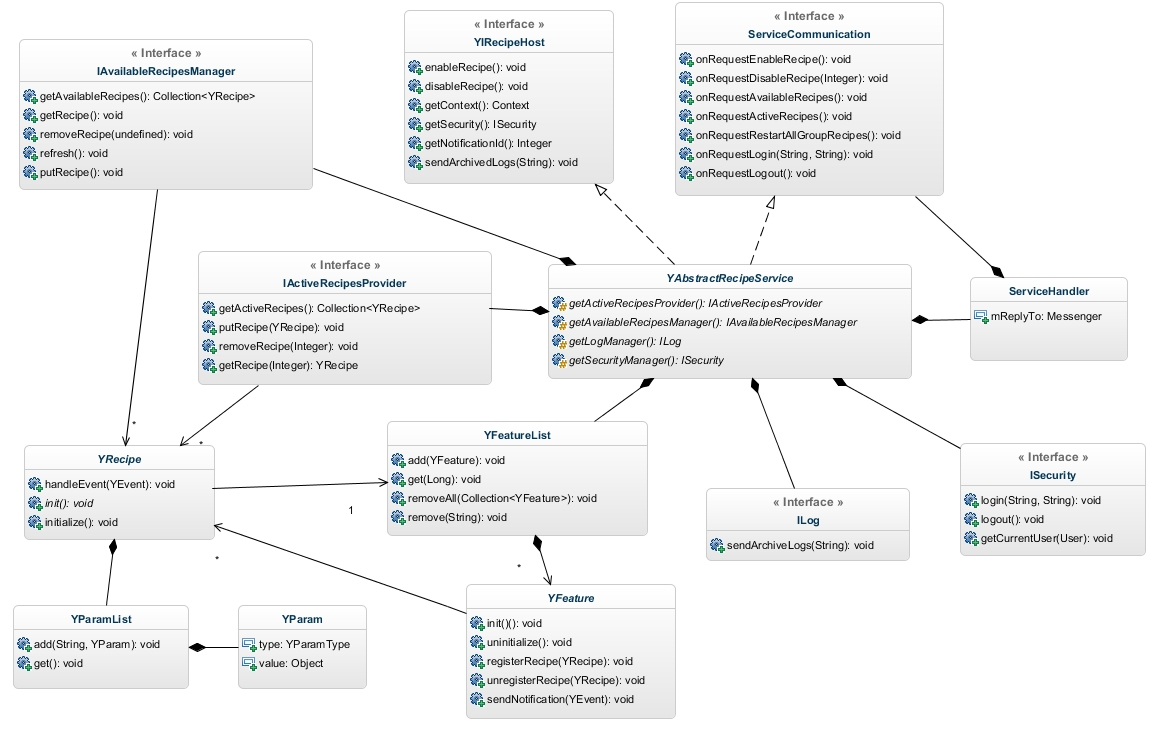
\includegraphics[scale=0.6]{./resources/service_uml.png}
  \caption{Diagram klas modułu zarządzania receptami}
  \label{fig:service_uml}
\end{figure}
Moduł zarządzania Receptami został zaimplementowany w klasie abstrakcyjnej YAbstractRecipeService, dziedziczącej po Serwisie.
Serwis w Androidzie to komponent aplikacji przeznaczony do długotrwałego wykonywania operacji w tle, nieposiadający interfejsu użytkownika. \cite{android.serwis}
Zaleca się uruchamianie Serwisu Biblioteki w osobnym procesie, dzięki czemu uruchomione Recepty mogą działać niezależnie od Aplikacji. Warto w tym miejscu nawiązać do zarządzania pamięcią w systemie Android - każda aplikacja uruchomiona przez użytkownika może zostać w dowolnym momencie zamknięta ze względu na konieczność zwolnienia zasobów. Serwis Biblioteki został zaimplementowany w taki sposób, aby być z powrotem uruchamiany po zamknięciu. Możliwe jest także uruchamianie go po starcie systemu.
Podczas projektowania tego modułu kluczowe było zapewnienie maksymalnego uproszczenia mechanizmów zarządzania Receptami z punktu widzenia programisty Aplikacji przy jednoczesnej dowolności implementacji list dostępnych i aktywnych Recept. Pozwoliło na stworzenie appIFY, w której użytkownik ma pełną kontrole nad modułem zarządzania, jak i wykorzystanie Biblioteki do napisania aplikacji wykorzystującej jedną wbudowaną Receptę, niewidoczną dla użytkownika końcowego.

\subsection{Podfunkcjonalności}
Podfunkcjonalności to klasy agregujące pewne funkcje związane z systemem. Muszą być inicjalizowane, gdy zajdzie taka potrzeba i przechwytywać zdarzenia systemowe, przekazując je odpowiednim receptom. Klasą bazową jest dla nich YFeature. Są w niej zaimplementowane metody związane z czasem życia Podfunkcjonalności i Recepty, odpowiedzialne za rejestrowanie i odrejestrowywanie Recept, inicjalizację i deinicjalizację Podfunkcjonalności oraz sprawdzanie, czy Podfunkcjonalność jest używana przez recepty. Poza tym znajduje się w niej metoda odpowiedzialna za wysyłanie zdarzenia do Recept - sendNotification, wykorzystywana w poszczególnych Podfunkcjonalnościach. Zaimplementowano następujące podfunkcjonalności:

\begin{itemize}
\item{Akcelerometr (YAccelerometerFeature.java)} \\
Umożliwia reagowanie na odczyty akcelerometru wbudowanego w urządzenie. 

\item{AudioManager (YAudioManager.java)}\\
Umożliwia zarządzanie poziomem głośności dzwonka.

\item{Battery (YBatteryFeature.java)}\\
Umożliwia reagowanie na zmiany poziomu baterii urządzenia.

\item{Calls (YCallsFeature.java)}\\
Umożliwia reagowanie na połączenia przychodzące i inicjowanie połączeń wychodzących.

\item{Files (YFilesFeature.java)}\\
Umożliwia tworzenie i odczytywanie plików z pamięci urządzenia lub nośnika zewnętrznego.

\item{Geocoder (YGeocoderFeature.java)}\\
Umożliwia pobranie adresu związanego z podaną długościa i szerokością geograficzną.

\item{GPS (YGPSFeature.java)}\\
Umożliwa śledzenie pozycji urządzenia za pomocą modułu GPS.

\item{Group (YGroupFeature.java)}\\
Niezbędny do obsługi zdarzeń grupowych.

\item{Intent (YIntentFeature.java)}\\
Pozwala wysyłać intencje\cite{android.intent} umożliwiające m. in. uruchamianie innych aplikacji.

\item{Internet (YInternetFeature.java)}\\
Umożliwia wysyłanie i pobieranie danych z podanego adresu.

\item{Notification (YNotificationFeature.java)}\\
Umożliwia wyświetlanie powiadomień w interfejsie graficznym urządzenia.

\item{RawPlayer (YRawPlayerFeature.java)}\\
Umożliwia odtwarzanie dźwięków na podstawie tablicy częstotliwości.

\item{Shortcut (YShortcutFeature.java.java)}\\
Pozwala na tworzenie skrótów do Recepty na głównym ekranie.

\item{SMS (YSMSFeature.java)}\\
Umożliwia wysyłanie wiadomości SMS oraz reagowanie na wiadomości przychodzące.

\item{Sound (YSoundFeature.java)}\\
Pozwala odtrzarzać pliki dźwiękowe.

\item{Text (YTextFeature.java)}\\
Umożliwia wprowadzanie tekstu do recepty z poziomu aplikacji.

\item{Time (YTimeFeature.java)}\\
%TODO Działa to?

\item{Wifi (YWifiFeature.java)}\\
Umożliwia włączanie i wyłączanie modułu WiFi urządzenia.

\end{itemize}

\subsection{Dziennik}
Biblioteka posiada moduł dziennika, pozwającego na zapisywanie i wyświetlanie informacji. Dostęp do niego miał przypominać jak najbardziej klasę Log \cite{android.log} w Androidzie. Powstała zatem klasa YLog zawierająca między innymi statyczne metody v,d,i,w,e, identyczne jak w Androidzie. Wywołują one swoje odpowiedniki, aby umożliwić debugowanie poprzez narzędzie logcat. Oprócz tego są wpisy są przechowywane wewnętrznie.
Do ich wyświetlania służy specjalny widok, wyświetlany jako nakładka. Nie reaguje on na dotyk, przez co umożliwia użytkowanie telefonu gdy jest widoczny. Jest to jedyny widok obsługiwany przez Bibliotekę, a nie Aplikacje Klienckie.
Dodatkowo istnieje klasa YLogger, której instancje są przypisane do recepty. Wpisy przez nią utworzone są przypisane do konkretnej Recepty. Dzięki temu można je łatwo odfiltrować i wyświetlać na ekranie Recepty w Aplikacji Klienckiej. 
Recepty mają do niej dostęp poprzez pole Log -- jego nazwa wydaje się przeczyć konwencji, jednak przypomina dzięki temu oryginalną klasę Log ze statycznymi metodami. Jedyną różnicą są argumenty metod -- zamiast taga i wiadomości przyjmowana jest jedynie wiadomość, tag jest tworzony automatycznie na podstawie Recepty.
\begin{figure}[H]
  \centering
  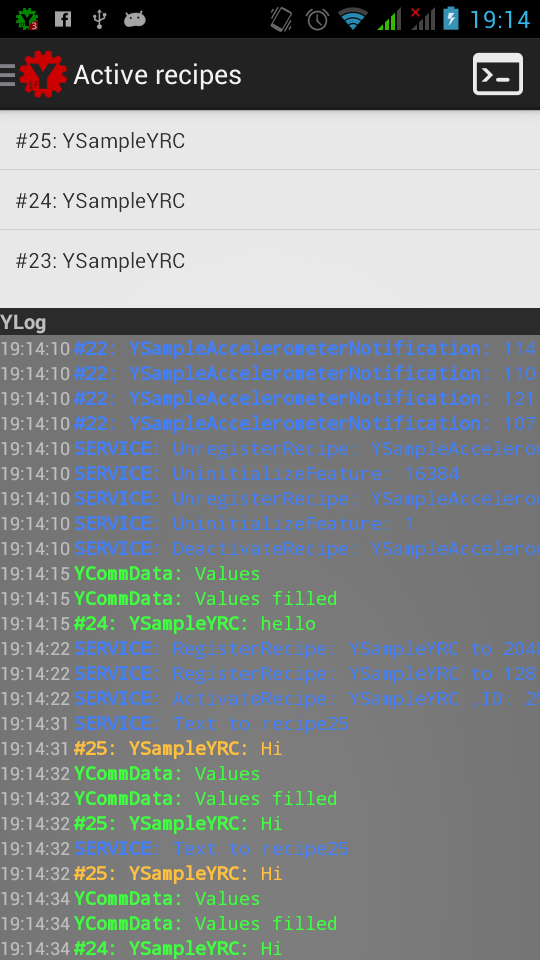
\includegraphics[scale=0.3]{./resources/logs.png}
  \caption{Widok dziennika nad ekranem Aplikacji Klienckiej}
  \label{fig:market_tree}
\end{figure}

\section{Aplikacja kliencka}
\subsection {Obsługa Targowiska}
Moduł obsługi Targowiska jest odpowiedzialny za  wyświetlanie danych dotyczących recept dodanych w aplikacji internetowej oraz pobieranie plików .jar ze skompilowanymi receptami, które następnie są zapisywane na pamięci wewnętrznej urządzenia mobilnego (w celu zachowania tej samej bazy recept w przypadku w którym użytkownik usunie zewnętrzny nośnik pamięci z urządzenia). Informacje o plikach z receptami (ich nazwy oraz ścieżki) przechowywanymi na telefonie zapisywane są po pomyślnym pobraniu w  bazie danych.
\subsection {Obsługa pobranych Recept}
W aplikacji klienckiej zrealizowanej w ramach pracy inżynierskiej rozróżniamy dwa typy recept - wbudowane i pobrane z Targowiska. Kod źródłowy recept pierwszego typu jest zawarty w kodzie źródłowym Aplikacji. W przypadku recept pobranych z Targowiska, w celu umożliwienia Aplikacji korzystania z takiej recepty wykorzystywane jest archiwum .jar, zawierające plik .dex (Dalvik Executable) z kodem wykonywalnym  zrozumiałym dla maszyny wirtualnej Dalvik. Informacje potrzebne do załadowania kodu recepty (nazwa klasy oraz ścieżka dostępu do pliku .jar) przechowywane są w bazie danych recept pobranych na urządzenie. 
\subsection{Komunikacja serwisu z aplikacją kliencką}
W opisie komunikacji między aplikacją kliencką a serwisem recept wykorzystane będą klasy z Android SDK - Messenger, Bundle i interfejs Parcelable. Klasa Messsenger umożliwia przesyłanie danych między procesami. \cite{android.mesage} Do opakowania danych wykorzystywana jest klasa Bundle, która przechowuje obiekty i typy prymitywne w postaci mapy. Warto wspomnieć, że aby uzyskać możliwość przechowania obiektu w tej klasie, musi on implementować interfejs Serializable lub Parcelable. Pierwszy z nich umożliwia serializacje obiektów znaną z Javy, natomiast drugi został zaimplementowany w Android SDK w celu zwiększenia wydajności serializacji. W pracy inżynierskiej wykorzystujemy drugi z mechanizmów. Po uruchomieniu serwis recept wystawia obiekt implementujący interfejs IBinder służący do wiązania obiektów klasy Activity z obiektami klasy Service,  z którym z kolei jest związany obiekt klasy Messenger zaimplementowany w serwisie recept. Aby ustanowić połączenie, Aktywność musi stworzyć obiekt klasy Intent, sparametryzować go klasą Service z którą nawiązywane jest połączenie i zapewnić obiekt implementujący interfejs ServiceConnection, który reaguje na uzyskanie i zerwanie połączenia, a następnie wywołać metodę bindService jako parametr podając wspomniany wyżej obiekt klasy Intent. Po nawiązaniu połączenia następuje wymiana obiektów klasy Messenger, dzięki czemu możliwa jest komunikacja w obie strony. Warto dodać, że ten mechanizm komunikacji jest asynchroniczny. Wiadomości wysyłane przez klasę Messenger odbierane są przez klasę Handler, ich zawartość jest interpretowana dzięki wysyłanemu kluczowi, a następnie dane są przekazywane serwisowi recept lub aktywności aplikacji klienckiej w celu dalszego przetwarzania. W pracy inżynierskiej wykorzystano dwie klasy dziedziczące po klasie Handler - ServiceHandler dla obsługi wiadomości przychodzących do serwisu recept i ActivityHandler dla obsługi wiadomości przychodzących do aplikacji klienckiej. W celu rozszerzenia komunikacji o wiadomości których obecna implemetnacja nie przewiduje, należy stworzyć własną klasę dziedziczącą po klasie ServiceHandler i we własnej implementacji klasy YAbstractService nadpisać metodę getServiceHandler. Podobnie, aby rozszerzyć komunikację w drugą stronę należy stworzyć własną klasę dziedziczącą po ActivityHandler i użyć go do odbierania wiadomości od serwisu recept.
\section{Targowisko}
Targowisko zaimplementowano w formie aplikacji internetowej. Łączy ono w sobie technologie takie jak PHP, MySQL, HTML, CSS oraz JavaScript. Jedyną różnicą w stosunku
do przeciętnych stron internetowych jest integracja z systemem operacyjnym poprzez skrypty powłoki BASH.

Targowisko ma trzy cele:
\begin{enumerate}
\item Zapewnić prosty w użyciu interfes użytkownika.
\item Udostępnić zunifikowany interfejs programowania aplikacji (API) który pozwoli uzyskać dostęp do wszystkich informacji z bazy danych.
\item Dać dostęp do skryptów powłoki BASH oraz zapewnić im bezpieczne wykonanie.
\end{enumerate}

W kontekście celów oraz technologii, jako wzór postępowania przyjęto wzorzec projektowy Model-Widok-Kontroler (MVC). Z racji na swoje organizacyjne właściwości, jest
on najlepszym wyborem pozwalającym oddzielić logikę od interfejsu.
\subsection{Wzorzec MVC}
\begin{figure}[H]
  \centering
  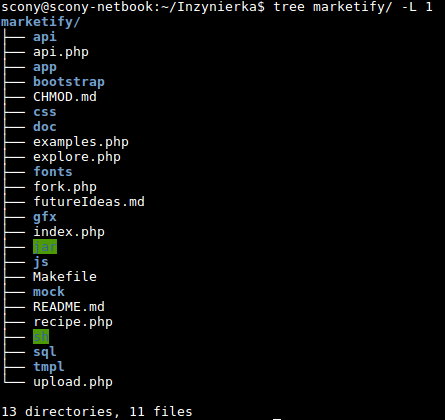
\includegraphics[scale=0.7]{./resources/market_tree.png}
  \caption{Struktura katalogowa targowiska}
  \label{fig:market_tree}
\end{figure}
Poprzez użycie Wzorca MVC w targowisku, uniemożliwiono technologiom mieszanie się ze sobą. Zjawisko takie jest częstym błędem popełnianym przez twórców aplikacji
internetowych. Utrudnia ono w znacznym stopniu rozwój oraz pielengnację kodu. Konsekwencje użycia wzorca MVC, widać najwyraźniej w strukturze katalogowej.
Prezentuje ją rysunek \ref{fig:market_tree}.
W głównym katalogu targowiska znajdują się pliki o rozszerzeniu \emph{php}. Są to kontrolery przetwarzające dane pochodzące od użytkownika. Pozostałe kontrolery
znajdują się w podkatalogu \emph{api}. Mają one na celu przetwarzenie żądań kierowanych do API.

Widoki znajdują się w katalogu \emph{tmpl}. Ich poprawne działanie jest jednak gwarantowane poprzez style oraz skrypty zgromadzone kolejno w podkatalogach
\emph{css} oraz \emph{js}.

Modele znaleźć można w podkatalogach \emph{app} oraz \emph{sql}.

\subsection{Interfejs graficzny}
Do realizacji graficznego interfejsu użytkownika użyto darmowy framework; Twitter Bootstrap. Jest to obszerny zbiór stylów CSS wraz z rzetelną dokumentacją. Pozwala on
osobie nie będącej uzdolnionej artystycznie, tworzyć dobrze wyglądające widoki aplikacji.

Framework jest bardzo prosty w użyciu. Po pierwsze, należy dołączyć jego pliki do struktury katalogowej swojej aplikacji. Po drugie, do kodu HTML należy dodać
następującą linię:
\begin{verbatim}
<link href="./css/bootstrap.css" rel="stylesheet">
\end{verbatim}

Aby przykładowo utworzyć efektywne menu, do znacznika UL będącego kontenerem dla hiperłączy wystarczy dodać odpowiednie klasy tak jak w przykładzie poniżej:
\begin{verbatim}
<ul class="nav nav-pills pull-right">
	<li><a href="explore.php">Recipes</a></li>
	<li><a href="examples.php">Examples</a></li>
	<li><a href="upload.php">Upload</a></li>
	<li><a href="doc" target="_blank">Doclava</a></li>
	<li><a href="api.php">API</a></li>
</ul>
\end{verbatim}

Dla lepszego wyobrażenia możliwości oferowanych przez framework, wystarczy spojrzeć na rysunek \ref{fig:market}.
\begin{figure}[p]
  \centering
  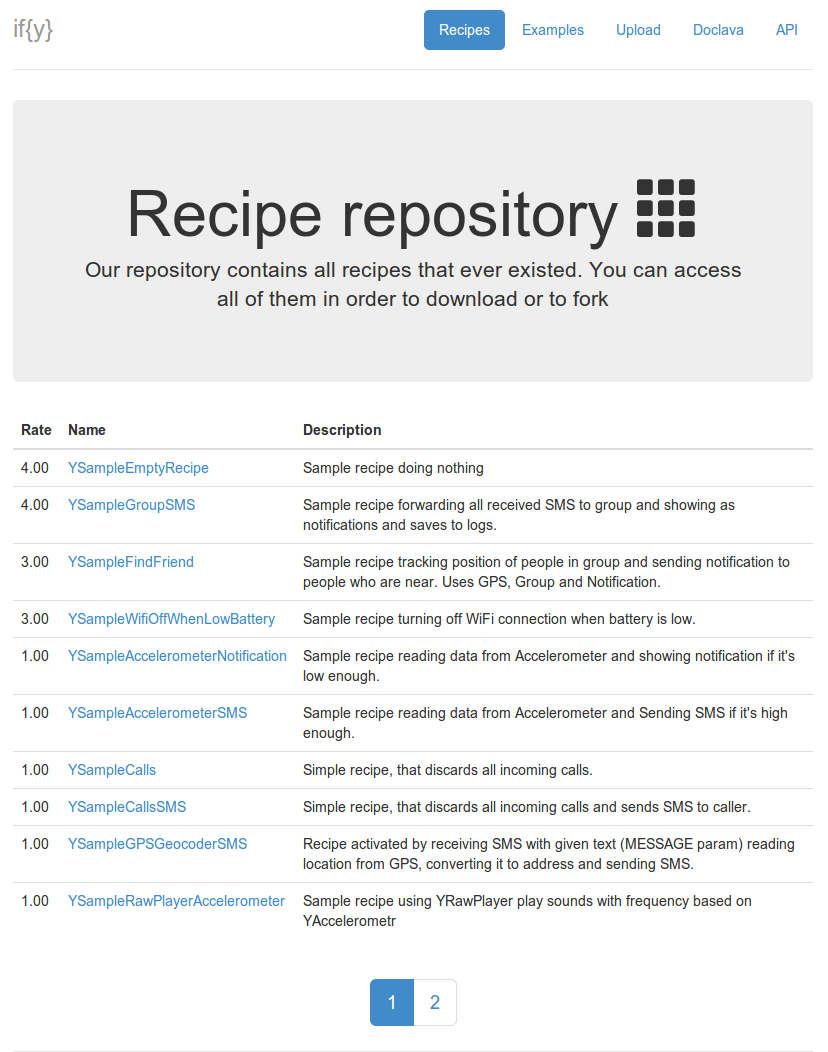
\includegraphics[scale=0.5]{./resources/market.png}
  \caption{Framework Twitter Bootstrap zastosowany do widoku listy recept targowiska}
  \label{fig:market}
\end{figure}
\subsection{Edytor Ace}
\begin{figure}[p]
  \centering
  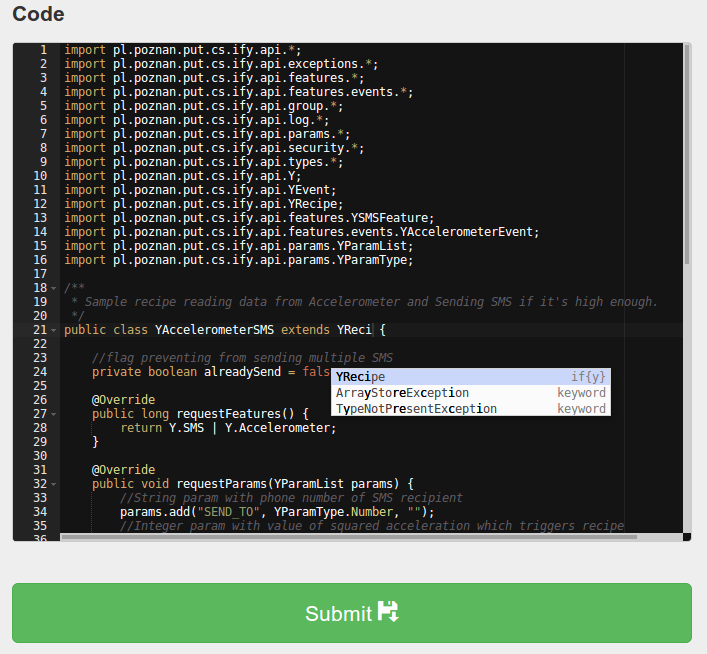
\includegraphics[scale=0.6]{./resources/market_ace.png}
  \caption{Edytor Ace oferuje między innymi kolorowanie składni oraz autouzupełnianie}
  \label{fig:market_ace}
\end{figure}
W celu umożliwienia pisania kodu recept z poziomu targowiska, skorzystano z darmowego edytora Ace. Jest to narzędzie dające możliwości znane z popularnych narzędzi
takich jak Vim czy Eclipse (rysunek \ref{fig:market_ace}). Napisano je w JavaScript, przez co osadzenie go we własnej aplikacji internetowej ogranicza się do
modyfikacji wyłącznie widoków.

Kod edytora należy najpierw dołączyć do kodu widoku. Można to zrobić dwojako; poprzez dołączenie plików edytora do struktury katalogowej lub poprzez dołączenie kodu
edytora ze zdalnej lokalizjacji. W targowisku skorzystano z drugiej możliwości:
\begin{verbatim}
<script src="http://ace.c9.io/build/src-min/ace.js" type="text/javascript"">
</script>
<script src="http://ace.c9.io/build/src-min/ext-language_tools.js" type="text/javascript">
</script>
\end{verbatim}
Pierwsze dwie linie tyczą się samego edytora. Pozostałe dwie dołączają rozszerzenie używane w targowisku celem uzyskania autouzupełniania widocznego na
rysunku \ref{fig:market_ace}.

Samo dołączenie kodu nie wystarcza do działania edytora. W treści strony trzeba dodać znacznik \emph{pre} o odpowiednim parametrze id:
\begin{verbatim}
<pre id="editor"></pre>
\end{verbatim}

Na koniec wykonać należy prosty skrypt JavaScript który uruchomi edytor wraz z rozszerzeniem:
\begin{verbatim}
var langTools = ace.require("ace/ext/language_tools");
var editor = ace.edit("editor");
editor.setOptions({enableBasicAutocompletion: true});
editor.setTheme("ace/theme/twilight");
editor.session.setMode("ace/mode/java");
var ifyCompleter = {
    getCompletions: function(editor, session, pos, prefix, callback) {
        $.getJSON(
          "./api/completer.php" + (prefix.length === 0 ? "" : "?prefix=" + prefix),
          function(wordList) {
      callback(null, wordList.map(function(ea) {
          return {name: ea.word, value: ea.word, score: ea.score, meta: "if{y}"}
                }));
          });
    }
}
langTools.addCompleter(ifyCompleter);
\end{verbatim}
\subsection{API}
Jako alternatywną dla interfejsu użytkownika metodę dostępu do danych, w targowisku zaimplementoano interfejs API. Jest on dedykowany aplikacjom na urządzenia mobilne.
Pracuje w trybie tylko do odczytu, dzięki czemu nie występuje ryzyko ingerencji w dane.

Działanie API opiera się o wywołania GET protokołu HTTP. Dane będące wynikiem wywołania zwracane są w formie wielowymiarowej tablicy zapisanej w formacie JSON. API
targowiska wyróżnia pięć możliwych żądań:
\begin{itemize}
\item O najnowsze recepty
\begin{itemize}
\item http://ADRES\_TARGOWISKA/api/new.php?limit=\{limit\}
\item \{limit\}, liczba naturalna -- ilość recept do pobrania
\end{itemize}
\item O wszystkie recepty
\begin{itemize}
\item http://ADRES\_TARGOWISKA/api/recipes.php?page=\{page\}\&limit=\{limit\}
\item \{page\}, liczba naturalna -- numer strony z której zostaną pobrane recepty
\item \{limit\}, liczba naturalna -- ilość recept przypadających na każdą stronę
\end{itemize}
\item O recepty których nazwy pasują do wzorca
\begin{itemize}
\item http://ADRES\_TARGOWISKA/api/search.php?phrase=\{phrase\}
\item \{phrase\}, łańcuch znaków -- wzorzec wyszukiwania
\end{itemize}
\item O konkretną receptę
\begin{itemize}
\item http://ADRES\_TARGOWISKA/api/recipe.php?name=\{name\}
\item \{name\}, łańcuch znaków -- pełna nazwa recepty
\end{itemize}
\item O losową receptę
\begin{itemize}
\item http://ADRES\_TARGOWISKA/api/random.php
\end{itemize}
\end{itemize}
Przykładowa odpowiedź targowiska na żądanie o losową receptę może wyglądać następująco:
\begin{verbatim}
[
   {
      "name":"YSampleYRC",
      "forked":null,
      "description":"Simple IRC - like chat, using YTextEvent, YGroupFeature and YLog.",
      "code":"(...)",
      "ts":1391197304,
      "safe":1,
      "url":"http:\/\/ADRES_TARGOWISKA\/jar\/YSampleYRC.jar",
      "rate":null,
      "comments":[

      ]
   }
]
\end{verbatim}
\subsection{Kompilacja Recept}
Po dodaniu recepty do bazy danych Targowiska jest ona kompilowana oraz przekształcana do wynikowego pliku \emph{jar} poprzez następujący skrypt powłoki BASH:
\begin{verbatim}
#!/bin/bash

if [ $# -eq 1 ];
then
    # clean
    rm -f recipe.jar
    # build
    javac -source 1.6 -target 1.6 -bootclasspath rt.jar -cp ify.jar:android.jar:rt.jar $1.java\
    || exit 1 # compability with jdk 1.6
    # javac -cp ify.jar:android.jar $1.java || exit 1
    jar cf tmp.jar $1.class
    ./dx --dex --output=classes.dex tmp.jar
    jar cf recipe.jar $1.class classes.dex
    # post-clean
    rm -f *.class
    rm -f classes.dex
    rm -f tmp.jar
    rm -f *.java
    exit 0
else
    echo 'Usage: ./build.sh [recipe class name without .java]'
    exit 2
fi
\end{verbatim}
\section{Serwer recept grupowych}
\subsection{Baza danych}
\begin{figure}[H]
  \centering
  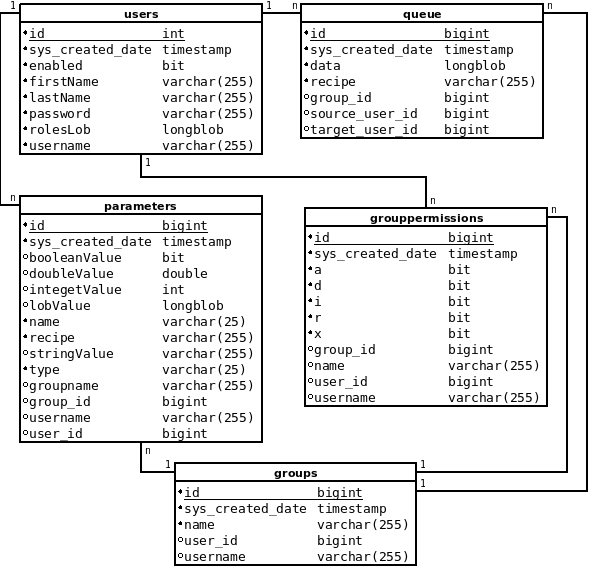
\includegraphics[scale=0.7]{./resources/server_db.png}
  \caption{Schemat bazy danych serwera grup}
  \label{fig:server_db}
\end{figure}
\subsection{Grupy i użytkownicy}
Łączenie użytkowników w grupy realizowane jest zapomocą relacji w bazie danych. 
Każda z grup jest opisana przez swoją unikalną nazwę dzieki której może być w łatwy sposób wyszukana, przy próbie utworzenia grupy o tej samej nazwie zostanie zwrócony wyjatek a z poziomu interfejsu bład walidacji.
Tabele reprezentujące grupy i użytkowników połaczone sa za pomoca tabeli pośredniej "groupspermmisions" w której zapisane sa informacje o uprawnieniach jakie posiada użytkownik w grupie. 
Uprawnienia nadawane sa dla kązdej grupy indywidualnie. 
Kazdy użytkownik w grupie posiada prawo do wypisywania listy uzytkowników w grupie ora tak prawo do wykonywania czyli możliwosć wysyłania wiadomości do innych uzytkowników w ramach tej grupy oraz zapisywanie własnych danych na serwerze.
Twórca grupy dodatkowo posiada wpis z uprawnieniem do dodawania nowych członków. 

\subsection{Uwierzytelnianie i autoryzacja} 
Po odebraniu każdej wiadomosci od uzytkonika jest on uwierzytelniany za pomocą loginu i hasła podanych w przypadku połączeń typu HTTP w JSONie lub dla połączeń typu REST w ścieżce URL.
W celu zapobiegnięcia przesyłaniu haseł w postaci jawnej, szyfrowane są one funkcją skrótu SHA-1.

Autoryzacja użytkownika odbywa się poprzez sprawdzenie uprawnień użytkownika do grupy którą podał w danych do komunikacji. 
Jako pierwsze sprawdzane jest czy użytkownik jest członkiem grupy, w ramach której wysyła wiadomość. 
Jeżeli użytkowni nie nalezy do grupy nie posiada żadnyc uprawnień w ramach tej grupy.
Dostępnych jest 5 uprawnień jakie może posiadać użytkownik dla kazdej z grup do której należy:
%ladnie proszę, darxi
Uprawnienia reprezentowane są przez flagi:
\begin{itemize}
\item d (ang. delete) pozwala usuwać użytkowników z grupy
\item a (ang. add) pozwala dodawać nowych użytkowników
\item r (ang. read) pozwala odcztywać członków grupy oraz nie widzi grupy na zwojej liście grup do których nalerzy.
\item x (ang. execute) umożliwia wysyłanie i odbieranie wiadomości w ramach grupy.
\item i (ang. invitation) oznacza że użytkownik został zaproszony do grupy i nie potwierdził zaproszenia. Jeżeli ustawiona jest ta flaga pozostałe uprawnienia traktowane są jak by nie były ustawione. Uzytkownik może tylko potwierdzić lub odrzucić zaproszenie do grupy.
\end{itemize}
Dla zapytań typu REST w przypadku nieuwierzytelnionej, nieautorysowanej komunikacji lub w przypadku błedu zwracana jest wartość "false".
Przy komunikacji z użyciem protokołu HTTP zostaje wysłana odpowiedź ze statusem błedu.
\subsection{Kolejka komunikatów}
Serwer pośrednicząc w komunikacji odbiera wiadomości, które do czasu wysłania do klienta docelowego są zapisywane w bazie danych.
Wiadomość w bazie jest w formie zserializowanej do ciągu bajtów.
Z kazdej wiadomości która zostanie odebrana pobierane są informacje niesbędne do zapisania jej oraz późniejszego zidentyfikowania takie jak nazwy grupy, recepty, użytkownika docelowego i nadawcy.
\subsection{Zarządzanie grupami}
\subsection{Komunikacja z receptami}
Komunikacja recept z serwerem grup odbywa się za pomocą odpowiedniego zapytania do serwera:
\begin{itemize}
\item Adres docelowy: ADRES\_SERWERA/rest/recipe
\item Typ zapytania: POST
\item Content-Type: application/json
\end{itemize}

W ciele zapytania znajduje się JSON o następującej strukturze:
\begin{verbatim}
{
    "user": {
        "username": STRING,
        "recipe": STRING,
        "group": STRING,
        "password": STRING
    },
    "event": {
        "target": STRING,
        "tag": INT
    },
    "values": {
        STRING: {
            "value": OBJECT,
            "type": STRING
        },
        STRING: {
            "value": OBJECT,
            "type": STRING
        },
       [...]
    }
}
\end{verbatim}

Oczywiście wyrazy pisane wersalikami to typy danych, których wartości są zależne od konkretnego zapytania.

Pole user ma na celu identyfikację nadawcy wiadomości - zawiera on nazwę użytkownika, recepty i grupy. Znajduje się tutaj także hasło, a ściślej - skrót SHA-1 hasła używający loginu jako soli. 

Pole event to login użytkownika do którego skierowany jest komunikat lub wartość specjalna BROADCAST oznaczająca skierowanie do wszystkich oraz tag określający typ zdarzenia.

Pole values to wartości przesłane wraz ze zdarzeniem. Mają formę słownika indeksowanego ciągami znaków. Każdy obiekt ma typ i wartość. Typy są tożsame z typami zdefiniowanymi w klasie YParamType, przy czym przy przesyłaniu JSON-en wartości typów innych niż Integer i Boolean są zamieniane na String.

Taki schemat danych odpowiada podstawowej operacja - sendEvent. Tag jest wówczas dodatni.
Pozostałe operacje jednak posługują się tym samych schematem z drobnymi różnicami:
\begin{itemize}
\item{sendValues} \\
Tag jest równy stałej YCommand.SEND\_DATA = 0. Pole event.target jest ignorowane. Nazwy tych danych różnią się od tych określonych w recepcie - mają formę nazwa@użytkownik, co zapewnia ich unikalność kluczy przy pobieraniu przez getAllValues. Oczywiście znak @ nie może być częścią loginu użytkownika, co jest weryfikowane przy rejestracji. 
 \item{getValues} \\
Tag jest równy stałej YCommand.GET\_DATA = -1. Pole event.target to użytkownik, którego dane nas interesują. W przypadku pustej wartości serwer zwraca dane całej grupy (operacja getAllValues). Pole values jest ignorowane.
\item{poll} \\
Tag jest równy stałej YCommand.POOLING = -4. Jest to techniczna operacja odpytywania serwera o zdarzenia kierowane do recepty. Pola event.target oraz values są ignorowane.
\end{itemize}
Odpowiedzi na żądania, jeśli wymagają przesłania danych są przekazywane w podobnej formie.
W wypadku zdarzeń pole user identyfikuje nadawcę. Oczywiście jest z niego usuwane pole password. Pola event i values są takie, jak w wiadomości tworzącej zdarzenie. 
Przy odpowiedziach na GET\_DATA pole values jest wypełnione wartościami danych zapisanymi na serwerze. Pola user i event są kopią tych wysłanych, jednak ich wartość jest ignorowana. 
\section{Użyte technologie}
W tej części zaprezentowano opis technologii użytych bezpośrednio w implementacji składowych platformy.
\begin{itemize}
\item{Android} \\
System operacyjny z rodziny Linux przeznaczony dla urządzeń mobilnych. Aktualnie rozwijane przez sojusz biznesowy Open Handset Alliance.
\item{Android SDK} \\
Platforma programistyczna umożliwiająca tworzenie aplikacji dla systemu Android. Zawiera wtyczkę do środowiska Eclipse, narzędzia wspierające prace programisty, emulator i biblioteki potrzebne do zbudowania aplikacji. Programy dedykowne platformie pisane są w języku Java i uruchamiane na maszynie wirtualnej Dalvik.
\item{Apache Commons} \\
\item{Apache HTTP Server} \\
\item{Git} \\
Rozproszony oraz wieloplatformowy system kontroli wersji będący wolnym oprogramowaniem. 
\item{HTML 5} \\
\item{Hibernate} \\
Narzędzie odwzorowań obiektowo-relacyjnych (ang. object-relation mapping, ORM) rozwijany na zasadzie wolnego oprogramowania. Umożliwia odworowania obiektowo-relacyjne, pamięć podręczną, leniwe (ang. Lazy loading), chciwe pobieranie oraz rozproszoną pamięć podręczną.
\item{JSON} \\
Skrót od JavaScript Object Notation. Jest to lekki, tekstowy format wymiany danych niezależny od języka programowania. Został wybrany ze względu na swoją czytelność i wsparcie ze strony bibliotek programistyzcnych.
\item{Java} \\
\item{JavaScript} \\
Skryptowy język oprogramowania stosowany na stronach internetowych.
\item{Apache Maven} \\
Narzędzie automatycznego budowania oprogramowania dla języka JAVA. Głównymi problemami jakie rozwiązuje Maven przy budowaniu aplikacji są: zarządzanie zależnościami, mozliwość wieloma modułami, wsparcie dla testów.
\item{MySQL} \\
System zarządzania relacyjnymi bazami danych. Jest to wolne oprogramowanie szczególnie upodobane przez twórców aplikacji internetowych. Bardzo dobrze współpracuje z językami takimi jak PHP czy Java
\item{PHP} \\
Obiektowy język programowania dedykowany generowaniu stron internetowych w czasie rzeczywistym. Szczególnie użyteczny w przypadku tworzenia prototypów tudzież niewielkich projektów wymagających stosunkowo niskiego poziomu abstrakcji.
\item{RESTeasy} \\
Framework oprogramowania służacy do tworzenia aplikacji rozproszonych, oparty na wzorcu architektury oprogramowania Representational State Transfer(REST).
\item{SpringFramework} \\
Framework(Szkielet) tworzenia aplikacji w języku Java a w szczególności JavaEE. Do najważniejszych fukcji Springa zalicza się wstrzykiwanie zależności (ang. dependency injection, DI) oraz programowanie aspektowe (ang. aspect-oriented programming, AOP).  
\item{Vaadin} \\
Framework sieciowy służący do tworzenia aplikacji sieciowych w szczególnosci interfejsu użytkownika w oparciu o Google Web Toolkit (GWT) w języku JAVA.
\item{JUnit} \\
Biblioteka służaca do tworzenia testów jednostkowych w jezyku Java.
\end{itemize}
\section{Użyte narzędzia}
\begin{itemize}
\item{Apache Tomcat} \\
Kontener aplikacji sieciowych.
\item{Eclipse} \\
Popularne zintegrowane środowisko programistyczne (IDE) wspierające głównie język Java (wtyczki pozwalają obsługiwać inne języki). 
\item{Android developer tools} \\
Wtyczka do Eclipse pozwalająca tworzyć aplikacje androidowe. Dodaje takie funkcjonalności jak edycja plików XML odpowiadających za wygląd aplikacji (również w trybie graficznym) czy debugowanie na telefonach oraz emulatorze.
\item{String Tool Suite} \\
Zintegrowane środowisko programistyczne oparte o Eclipsa dostosowany do SpringFramework.
\item{Emacs} \\
Popularny, w pełni rozszerzalny edytor tekstowy spotykany głównie w systemach operacyjnych z rodziny Unix.
\item{Git bash for windows} \\
Narzędzie umożliwiające używanie Gita z linii poleceń w systemie Windows poprzez wbudowane środowisko MinGW.
\item{Github} \\
Serwis internetowy gromadzący społeczność programistów z całego świata. Służy jako hosting dla otwartoźródłowych projektów zarządzanych za pomocą systemu Git.
Udostępnia szereg narzędzi wspierających - system śledzenia zadań, budowa statystyk.
\item{Latex} \\
\item{Linux} \\
Rodzina systemów operacyjnych będących wolnym oprogramowaniem oraz używajnących jądra Linux.
\item{Notepad++} \\
Prosty edytor tekstowy umożliwiający kolorowanie składni w wielu językach.
\item{Przeglądarki internetowe} \\
Google Chrome, Mozilla Firefox, Opera
\item{Windows} \\
\end{itemize}
\section{Urządzenia mobilne}
Aplikacja była testowana na następujących urządzeniach mobilnych:
\begin{itemize}
\item{LG Swift GT540} \\
Procesor: Qualcomm MSM7227 600 MHz
Pamięć RAM: 256 MB
System operacyjny: Android 4.0.1 (Cyanogen mod)
\item{Media-Droid IMPERIUS EN3RGY MT7013}
Procesor: dwurdzeniowy, 1GHz ARM7 MTK6577
Pamięć RAM: 256 MB
System operacyjny: Android 4.1.2
\item{Motorola Defy MB525} \\
Procesor: TI OMAP3610 800 MHz
Pamięć RAM: 512 MB
System operacyjny: Android 4.3.1 (Cyanogen mod)
\item{Sony LT18 Xperia Arc S} \\
Procesor: Qualcomm MSM8255T 1,40 GHz
Pamięć RAM: 512 MB
System operacyjny: Android 4.0.4
\item{Samsung Galaxy Mini GT-S5570} \\
Procesor: Qualcomm MSM7227 600 MHz
Pamięć RAM: 384 MB
System operacyjny: Android 2.2
\end{itemize}

\section{Opis pakietów}
\subsection{Pakiety Aplikacji}
pl.poznan.put.cs.ify.app - główny pakiet Aplikacji.
pl.poznan.put.cs.ify.jars - pakiet odpowiedzialny za zarządzanie plikami .jar zawierającymii recepty pobrane z Targowiska.
pl.poznan.put.cs.ify.core - pakiet odpowiedzialny za zarządzanie dostępnymi i aktywowanymi Receptami.
pl.poznan.put.cs.ify.appify.receipts - pakiet zawierający Recepty wbudowane w Aplikację.
pl.poznan.put.cs.ify.app.ui - pakiet zawierający kontrolki interfejsu użytkownik.
pl.poznan.put.cs.ify.app.ui.params - pakiet zawierający kontrolki interfejsu użytkownika wykorzystywane do wprowadzania parametrów przy inicjalizacji Recepty.
pl.poznan.put.cs.ify.app.market - pakiet odpowiedzialny za pobieranie danych z Targowiska i wyświetlanie ich.
pl.poznan.put.cs.ify.app.fragments - pakiet zawierający widoki ekranów aplikacji.
\subsection{Pakiety Biblioteki}
pl.poznan.put.cs.ify.api - pakiet główny Biblioteki.
pl.poznan.put.cs.ify.api.exceptions - pakiet zawierający wyjątki, które mogą być rzucane przez metody z Biblioteki.
pl.poznan.put.cs.ify.api.features - pakiet zawietający Podfunkcjonalności i Zdarzenia.
pl.poznan.put.cs.ify.api.group - pakiet odpowiedzialny za obsługę Recept Grupowych.
pl.poznan.put.cs.ify.api.log - pakiet odpowiedzialny za obsługę logowania i domyślny widok logów.
pl.poznan.put.cs.ify.api.params - pakiet zawierający typy parametrów wykorzystywanych przez Recepty.
pl.poznan.put.cs.ify.api.security - pakiet odpowiedzialny za moduł uprawnień Biblioteki.
pl.poznan.put.cs.ify.api.types - pakiet zawierający typy danych wykorzystywanych przez Biblioteke.
\subsection{Pakiety Serwera}
pl.poznan.put.cs.ify.webify - pakiet główny serwera.
pl.poznan.put.cs.ify.webify.data.dao - pakiet zawierający warstwe dostępu do danych.
pl.poznan.put.cs.ify.webify.data.entity - pakiet zawierający klasy odwzorowywane na bazę danych.
pl.poznan.put.cs.ify.webify.data.enums - pakiet zawierajacy potrzebne w bazie danych typy wyliczeniowe(np. lista ról). 
pl.poznan.put.cs.ify.webify.gui - pakiet główny graficznego interfejsu użytkownika.
pl.poznan.put.cs.ify.webify.gui.windows - paiet zawierający wszytskie okna aplikacji sieciowej.
pl.poznan.put.cs.ify.webify.gui.components - pakiet zawierający komponenty użyte w aplikacji.
pl.poznan.put.cs.ify.webify.gui.session - 
pl.poznan.put.cs.ify.webify.service - pakiet zawierający logikę.
pl.poznan.put.cs.ify.webify.rest - pakiet zawerajacy obsługę zapytań typu REST.
pl.poznan.put.cs.ify.webify.utils - pakiet, w którym przechowywane są funkcje pomocnicze używane w całym projkcie.

\chapter{Wyniki}
\section{Cykl życia recepty w praktyce}
W efekcie ukończenia prac nad wszystkimi modułami platformy, możliwym stało się odtworzenie cyklu życia recepty w praktyce. Użytkownik kompetentny do pisania
kodu w języku Java, jest od tego miejsca w stanie tworzyć recepty ograniczając się wyłącznie interfejsem biblioteki oraz własną wyobraźnią.

W dalszej części rozdziału, przedstawiona zostanie recepta informująca o wzajemnej bliskości osób należących do grupy oraz przeanalizowany zostanie każdy etap
jej cyklu życia.
\subsection{Pisanie kodu}
\begin{figure}[H]
  \centering
  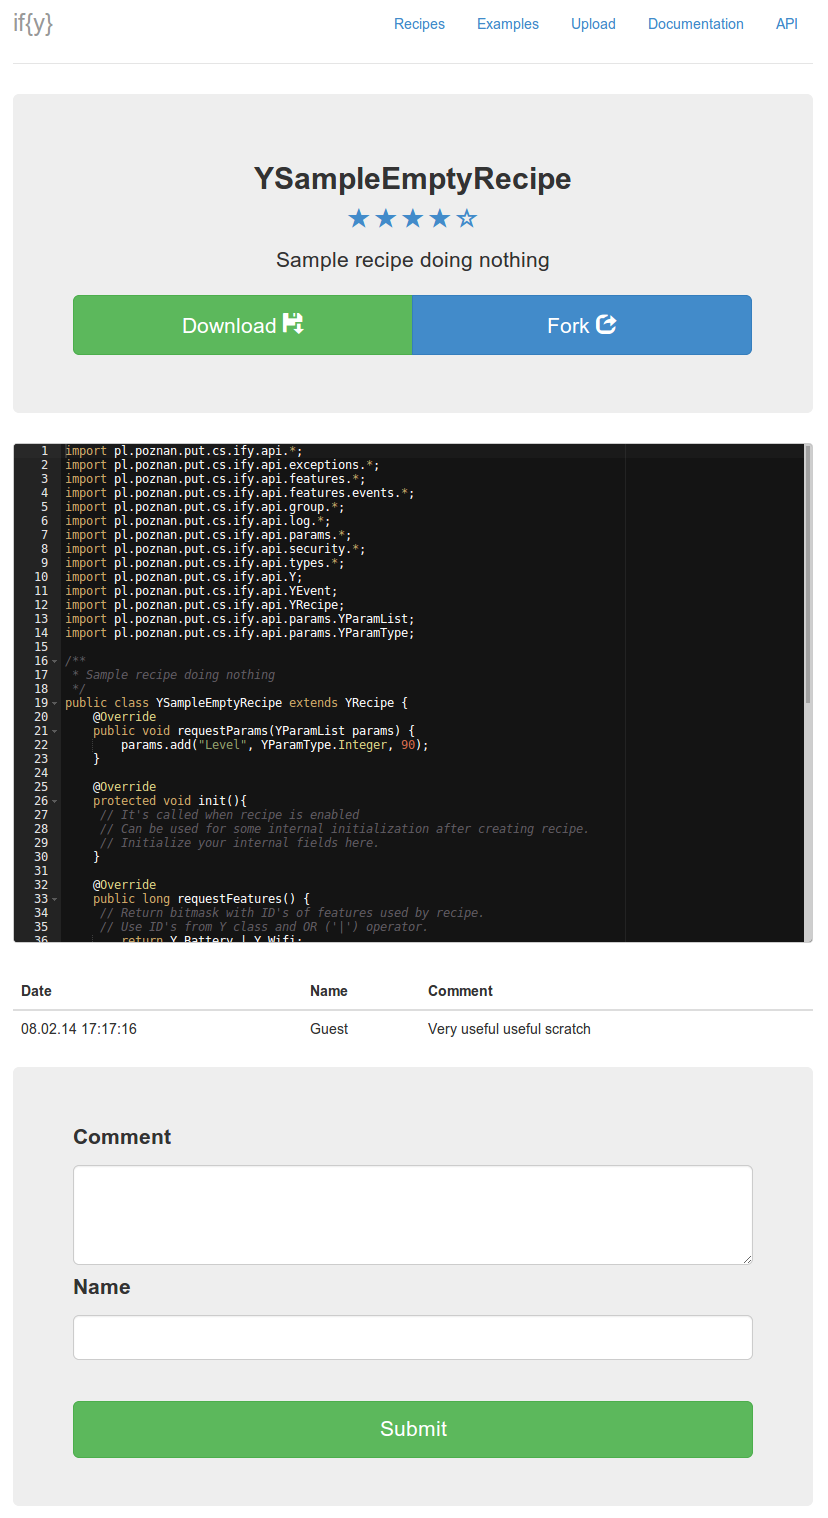
\includegraphics[scale=0.4]{./resources/market_recipe.png}
  \caption{Widok przykładowej recepty w targowisku}
  \label{fig:market_recipe}
\end{figure}
Pierwszym krokiem do napisania kodu własnej recepty jest zapoznanie się z przykładami dostępnymi na stronie targowiska w dziale \emph{examples}. Przykładowa recepta
może wyglądać jak na rysunku \ref{fig:market_recipe}. Każda przykładowa recepta to działający kod zawierający przydatne informacje zawarte w komentarzach. Gdy komentarze i przykłady nie wystarczą, sięgnąć należy do dokumentacji dostępnej w targowisku w dziale \emph{documentation}.

Po nabyciu niezbędnej wiedzy, najprościej zacząć od rozwidlenia gotowej recepty. Sprowadza się to do kliknięcia przycisku \emph{fork} z poziomu widoku recepty oraz
wprowadzenia nowej nazwy. Alternatywną drogą, jest rozpoczęcie pisania recepty od podstaw. W tym celu należy przejść do działu targowiska o nazwie \emph{upload}.

Pisanie kodu odbywa się w edytorze który szerzej opsiany został w rozdziale 5.5.3. W celu wywołania okna autouzupełniania należy użyć skrótu klawiszowego
\emph{CTRL+SPACJA}.
\subsection{Kompilacja i budowa}
Po zakończeniu pisania kodu wystarczy nacisnać przycisk \emph{submit} i odczekać kilka sekund.

\begin{figure}[H]
  \centering
  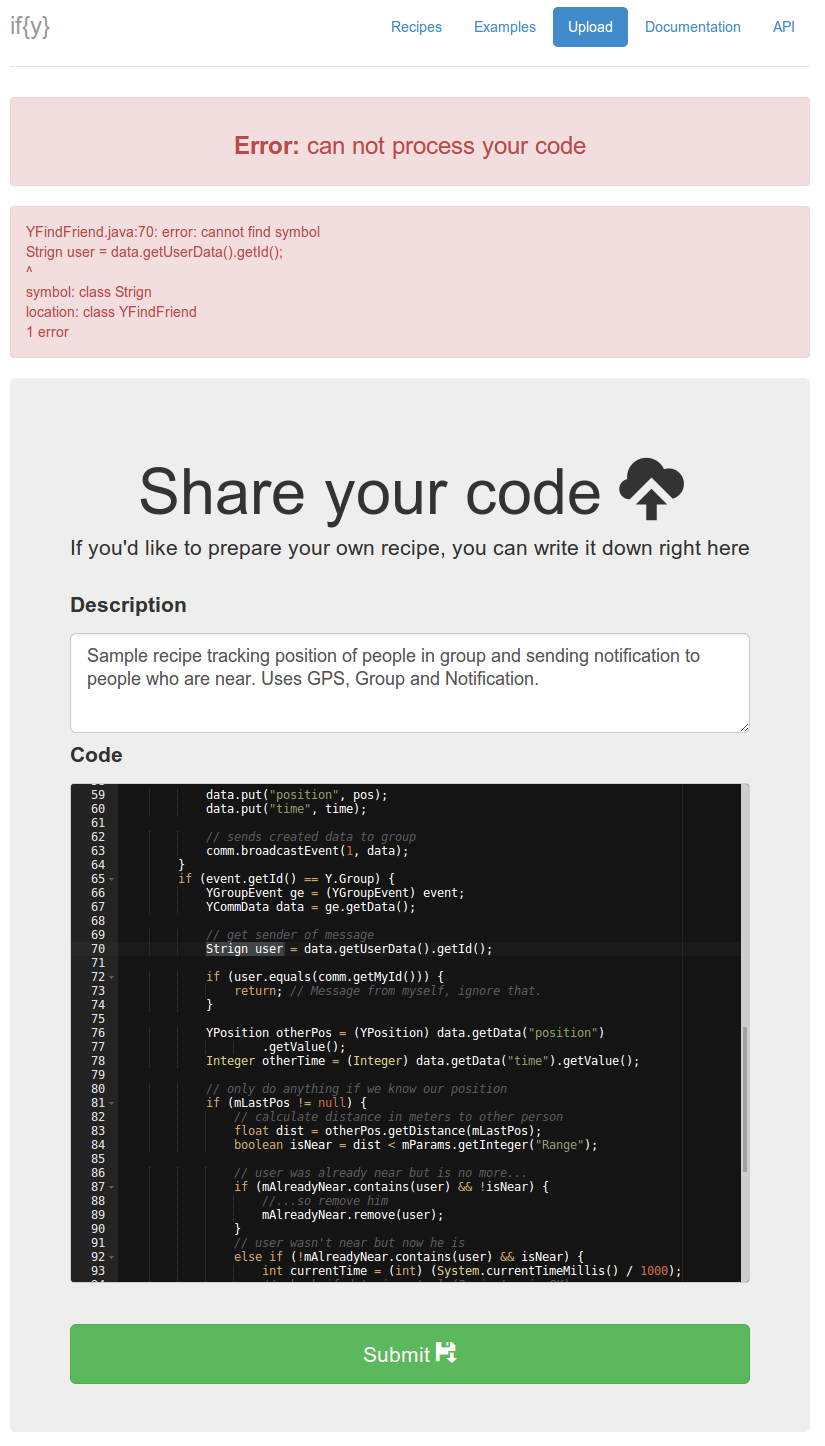
\includegraphics[scale=0.4]{./resources/market_error.png}
  \caption{Błąd w trakcie kompilacji kodu recepty}
  \label{fig:market_error}
\end{figure}
W przyapdku niepowodzenia etapu kompilacji czy budowy, użytkownik
dostaje pełną informację o błędzie jak na rysunku \ref{fig:market_error}. Po przeanalizowaniu komunikatu o błędzie, użytkownik może wprowadzić niezbędne zmiany oraz
ponownie nacisnać przycisk \emph{submit}.

W przypadku poprawnego przetworzenia kodu recepty, użytkownik zostaje przekierowany bezpośrednio do jej widoku.
\subsection{Dystrybucja}
Zbudowana poprawnie receptacepta dostępna jest natychmiastowo zarówno w targowisku jak i module targowiska aplikacji if\{y\} w urządzeniu mobilnym. Aby recepta
zdobyła popularność i uznanie wśród społeczności, warto aby jej kod był możliwie wysokiej jakości oraz z dużą ilością komentarzy.

O sukcesie recepty decydują oceny nadawane przez użytkowników oraz pozostawione przez nich komentarze.
\subsection{Pobranie na urządzenie mobilne}
\subsection{Uruchomienie}
\subsection{Działanie}

\chapter{Zakończenie}
\subsection{Podsumowanie}

\subsection{Dalszy rozwój (platformy)}

\appendix 

\section {Recipe creation guide}

Best way to create recipe is forking existing one from the market - just choose one from Examples or Recipes tab. Then you can edit it's code in browser. You don't have to care about ify imports - they will be added automatically when uploading recipe. More information is avaible in Doclava tab in market. \\*\\*
Currently market is avaible here:\\*\\*
http://ify.cs.put.poznan.pl/~scony/marketify\\*\\*
You can access some fields and methods generated by system which can be useful:\\*\\*
getParams()\\*
List of params requested in requestParams. It's populated with values when init() and handleEvent() code is called. Use getString(String name), getInteger(String name), etc. to get param with given name depanding what type param is.\\*\\*
getFeatures()\\*
Contains required features. Use specified getters like getSMS(), getWifi(), etc. or use general method get(Long id) inserting id from Y and cast returned feature to right type.\\*\\*
Log\\*
Use if to create logs with methods wtf(String), e(String), w(String), i(String), d(String), v(String). These logs will be visible on recipe screen and saved to Android logs (use LogCat to see it)\\*\\*
Here is quick overview of methods you need to implement in your recipe, you can find same information in YEmptyRecipe example.\\*\\*
protected void init()\\*
It's called when recipe is enabled, can be used for some internal initialization after creating recipe. Initialize your internal fields here.\\*\\*
public long requestFeatures()\\*
Return bitmask with ID's of features used by recipe. Use ID's from Y class and OR ('|') operator.\\*\\*
public void requestParams(YParamList params)\\*
Populate params object with definitions of needed params using params.add(String paramName, YParam param)\\*\\*
protected void handleEvent(YEvent event)\\*
It's place for main recipe logic. It's called on event connected with requested feature occurs. Check what event is that by checking event.getId() and compare it to id's from Y.\\*\\*
public String getName()\\*
Return String same like your recipe class name here. It's needed to avoid using reflection which is slow.\\*\\*
public YReceipt newInstance()\\*
Just call default constructor and return recipe instance. Also needed to avoid reflection.\\*\\*



\backmatter

\begin{thebibliography}{1}
%Jak się używa jednej ksiązki to jest plagiat ale jak wielu to jest poprostu bibliografia.
\bibitem{onx}Projekt on\{X\} http://www.onx.ms/\#!findOutMorePage. Ostatnio odwiedzone 6/02/13.
\bibitem{springinaction}C.~Walls. \emph{Spring in action, 3rd edition}. Manning Publication Co, 2011.
\bibitem{vaadinbook}Vaadin https://vaadin.com/book/vaadin6/-/page/preface.html 
\bibitem{patterns}E.~Gamma. \emph{Design Patterns, First edition}. Person Education, Inc, 1995.
\bibitem{java}The Reflection API  http://docs.oracle.com/javase/tutorial/reflect/index.html Ostatnio odwiedzone 31.01.2014
\bibitem{android.serwis} Android API Guide - Service http://developer.android.com/guide/components/services.html Ostatnio odwiedzone 31.01.2014
\bibitem{android.mesage} Android API Guide - Messenger http://developer.android.com/guide/components/bound-services.htmlMessenger  Ostatnio odwiedzone 31.01.2014 
\bibitem{android.intent} Android API Guide - Intents and Intent Filters http://developer.android.com/guide/components/intents-filters.html Ostatnio odwiedzone 31.01.2014 
\bibitem{android.log} Android API Guide - Reading and Writing Logs http://developer.android.com/tools/debugging/debugging-log.html Ostatnio odwiedzone 31.01.2014
\bibitem{googleplay}Introducing Google Play: All your entertainment, anywhere you go - http://googleblog.blogspot.com/2012/03/introducing-google-play-all-your.html Ostatnio odwiedzone 31.01.2014
\end{thebibliography}

\end{document}
